\documentclass[11pt]{article}
	\usepackage[T1]{fontenc}
    % Nicer default font (+ math font) than Computer Modern for most use cases
    % \usepackage{mathpazo}

    % Basic figure setup, for now with no caption control since it's done
    % automatically by Pandoc (which extracts ![](path) syntax from Markdown).
    \usepackage{graphics}
    % We will generate all images so they have a width \maxwidth. This means
    % that they will get their normal width if they fit onto the page, but
    % are scaled down if they would overflow the margins.
    \makeatletter
    \def\maxwidth{\ifdim\Gin@nat@width>\linewidth\linewidth
    \else\Gin@nat@width\fi}
    \makeatother
    \let\Oldincludegraphics\includegraphics
    % Set max figure width to be 80% of text width, for now hardcoded.
    \renewcommand{\includegraphics}[1]{\Oldincludegraphics[width=.8\maxwidth]{#1}}
    % Ensure that by default, figures have no caption (until we provide a
    % proper Figure object with a Caption API and a way to capture that
    % in the conversion process - todo).
    \usepackage[center,bf]{caption}
    % \DeclareCaptionLabelFormat{nolabel}{}
    % \captionsetup{labelformat=nolabel}

    \usepackage{adjustbox} % Used to constrain images to a maximum size 
    \usepackage{xcolor} % Allow colors to be defined
    \usepackage{enumerate} % Needed for markdown enumerations to work
    \usepackage{geometry} % Used to adjust the document margins
    \usepackage{amsmath} % Equations
    \usepackage{amssymb} % Equations
    \usepackage{textcomp} % defines textquotesingle
    % Hack from http://tex.stackexchange.com/a/47451/13684:
    \AtBeginDocument{%
        \def\PYZsq{\textquotesingle}% Upright quotes in Pygmentized code
    }
    \usepackage{upquote} % Upright quotes for verbatim code
    \usepackage{eurosym} % defines \euro
    \usepackage[mathletters]{ucs} % Extended unicode (utf-8) support
    \usepackage[utf8x]{inputenc} % Allow utf-8 characters in the tex document
    \usepackage{fancyvrb} % verbatim replacement that allows latex
    \usepackage{grffile} % extends the file name processing of package graphics 
                         % to support a larger range 
    % The hyperref package gives us a pdf with properly built
    % internal navigation ('pdf bookmarks' for the table of contents,
    % internal cross-reference links, web links for URLs, etc.)
    \usepackage{hyperref}
    \usepackage{longtable} % longtable support required by pandoc >1.10
    \usepackage{booktabs}  % table support for pandoc > 1.12.2
    \usepackage[inline]{enumitem} % IRkernel/repr support (it uses the enumerate* environment)
    \usepackage[normalem]{ulem} % ulem is needed to support strikethroughs (\sout)
                                % normalem makes italics be italics, not underlines
   	\usepackage[]{authblk}
   	\usepackage{cite}
    \usepackage{graphicx}
    \usepackage{hyperref}
    \usepackage{amsmath}
    \usepackage{amsthm}
    \usepackage{amssymb}
    \usepackage{bm}
    \usepackage{bbm}
    \usepackage{algorithmicx}
    \usepackage{algorithm}
    \usepackage{algpseudocode}
    \usepackage{array}
    \usepackage{booktabs}
    \usepackage{multirow}
    \usepackage{makecell}
    \usepackage{color}
    \usepackage{tabularx,ragged2e,booktabs,caption}

   	\makeatletter
    \def\@maketitle{%
    \newpage
      \null
      \vskip 2em%
      \begin{center}%
      \let \footnote \thanks
        {\Large\bfseries \@title \par}%
        \vskip 1.5em%
        {\normalsize
          \lineskip .5em%
          \begin{tabular}[t]{c}%
            \@author
          \end{tabular}\par}%
        \vskip 1em%
        {\normalsize \@date}%
      \end{center}%
      \par
      \vskip 1.5em}
    \makeatother


\newtheorem{theorem}{Theorem}






\title{EE 232E Project 4\\IMDb Mining}
\author{Hengjie~Yang, Sheng~Chang, Wandi~Cui, and Tianyi~Liu
}


\date{\today}


\begin{document}
\maketitle

% \section{A brief tutorial on how to use this template}
% \Large\textcolor{red}{\bf{Please remove the tutorial section in the final manuscript\\ by commenting, i.e. $\%(something)$}}


% \subsection{Figures}
% Figure insertion is shown in Fig \ref{example_fig}.
% \begin{figure}[h]
% \centering
% \scalebox{0.7}{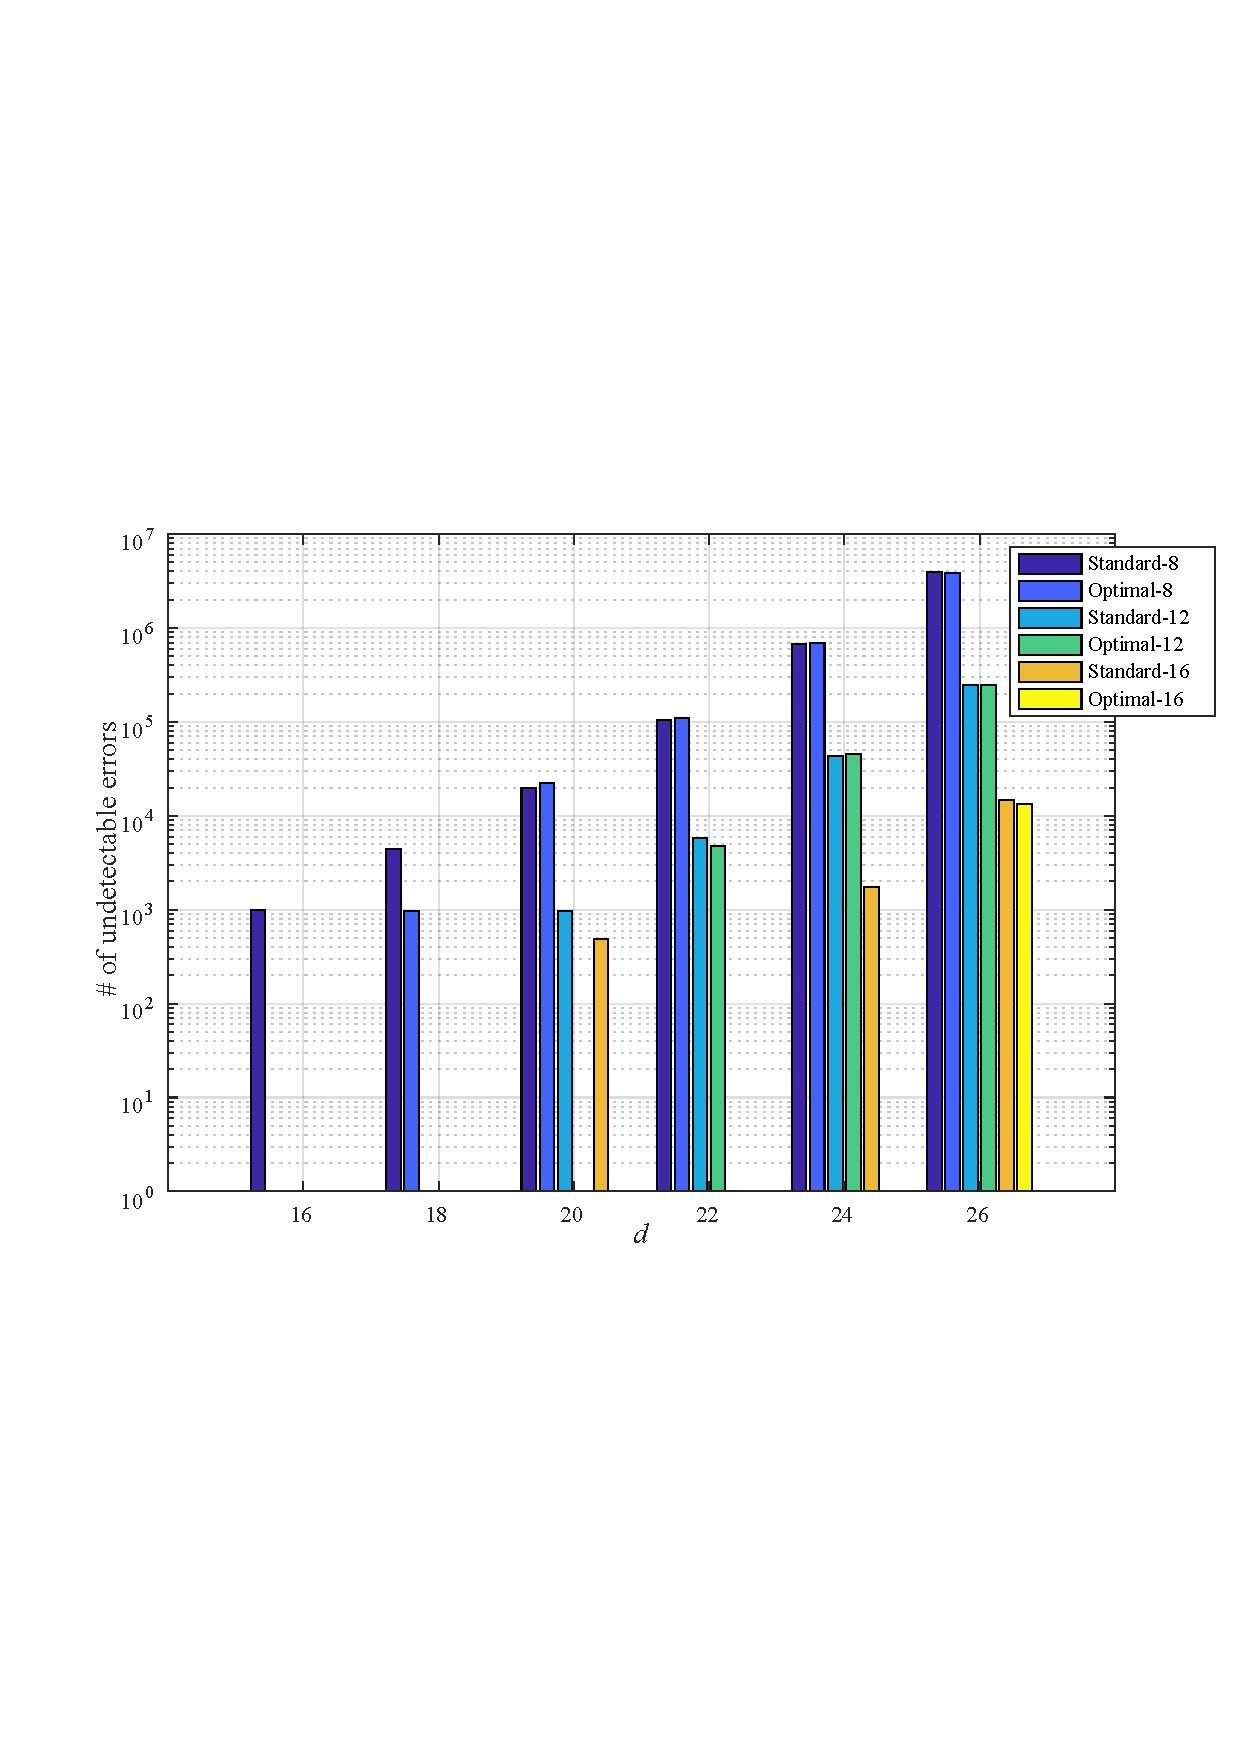
\includegraphics{Figures/spectrum_bar.pdf}}
% \caption{An example of figure insertion}
% \label{example_fig}
% \end{figure}

% \subsection{Equations}
% An example of equations is given as follows.
% \begin{theorem}
% Let $a$, $b$, $c$ denote the sides of a triangle, respectively. If $a\perp b$, the pythagoras theorem is given as follows.
% \begin{align}
% c^2 = a^2 + b^2
% \end{align}
% \end{theorem}

% \subsection{Tables}
% An example of tables is shown in Table \ref{example_table}.
% \renewcommand\arraystretch{1.1}
% \begin{table}[h]
% \center
% \caption{Standard CRC Codes versus Optimal CRC Codes for Convolutional Code $G=(561~753)$ with $n=504$ Bits}
% \scalebox{0.9}{
% \begin{tabular}{r|c|c|cccccc}
% \hline
% \multirow{2}{*}{Name} & \multirow{2}{*}{Gen. Poly.} & \multicolumn{7}{c}{Undetected Error Distance Spectrum} \\
% \cline{3-9}
%  & & $d$ & 16 & 18 & 20 & 22 & 24 & 26 \\\hline\hline
% Standard-8 & \multicolumn{1}{l}{0x19B} & & 983 & 4387 & 19909 & 105000 & 672724 & 3972970\\
% Optimal-8 & \multicolumn{1}{l}{0x19D} & & 0 & 979 & 22349 & 111304 & 686314 & 3830340\\\hline
% Standard-12 & \multicolumn{1}{l}{0x180F} & & 0 & 0 & 969 & 5815 & 42893 & 245211 \\
% Optimal-12 & \multicolumn{1}{l}{0x108B} & & 0 & 0 & 0 & 4793 & 45795 & 246729\\\hline
% Standard-16 & \multicolumn{1}{l}{0x11021} & & 0 & 0 & 484 & 0 & 1765 & 14752\\
% Optimal-16 & \multicolumn{1}{l}{0x1F8FD} & & 0 & 0 & 0 & 0 & 0 & 13240\\\hline
% \end{tabular}}
% \label{example_table}
% \end{table}

\section{Actor/Actress Network}

\subsection{Directed actor/actress network creation}

\subsection{Actor pairings}


\subsection{Actor rankings}
We aimed to find to find the top 10 actor/actress in the network using the google’s pagerank algorithm. Those information of the top 10 actor/actress is shown in Table \ref{table_1_3}, including the name, the number of movies and the in-degree of each of the actor/actress in the top 10 list.

\begin{table}
\center
\caption{Top 10 highest pagerank score actor/actress}
\scalebox{0.9}{
\begin{tabular}{r|c|c}
\hline
\textbf{Name} & \textbf{the Number of Movies} & \textbf{In-degree}\\\hline
Flowers, Bess & 828 & 7537\\\hline
Tatasciore, Fred & 355 & 3954\\\hline
Harris, Sam (II) & 600 & 6960\\\hline
Blum, Steve (IX) & 373 & 3316\\\hline
Miller, Harold (I) & 561 & 6587\\\hline
Jeremy, Ron & 637 & 3177\\\hline
Phelps, Lee (I) & 647 & 5563\\\hline
Lowenthal, Yuri & 318 & 2662\\\hline
Downes, Robin Atkin & 267 & 2953\\\hline
O'Connor, Frank (I) & 623 & 5502\\\hline 
\end{tabular}}
\label{table_1_3}
\end{table}

We can see from the result that it does not have any of the actor/actress listed in the previous section. In general, the more movie they took part in, the high pagerank they may had, because that means they had more changes to cooperate with other actor/actress and it's obvious that they may have higher degree in the network. After googling it, we found that most people int the top 10 are actually voice actors. That's why they can take part in hundreds of movies and that also explains why those famous previous actor/actress are not included in the top 10. Even though those movie super stars acted so many movies, it's very common that they still act less than those voice actors.

What's more, the same information of the actor/actress listed in the previous section is shown in Table \ref{table_1_4}.

\begin{table}[h]
\center
\caption{The same information table for previous actor/actress}
\scalebox{0.9}{
\begin{tabular}{r|c|c}
\hline
\textbf{Name} & \textbf{the Number of Movies} & \textbf{In-degree}\\\hline
Tom Cruise & 63 & 1651\\\hline
Emma Watson (II) & 25 & 453\\\hline
George Clooney & 67 & 1573\\\hline
Tom Hanks & 80 & 2064\\\hline
Dwayne Johnson (I) & 78 & 1357\\\hline
Johnny Depp & 98 & 2144\\\hline
Will Smith (I) & 49 & 1319\\\hline
Meryl Streep & 97 & 1594\\\hline
Leonardo DiCaprio & 49 & 1301\\\hline
Brad Pitt & 71 & 1739\\\hline

\end{tabular}}
\label{table_1_4}
\end{table}

\section{Movie Network}

\subsection{Undirected movie network creation}
We create a weighted undirected movie network. And the degree distribution of the movie network is shown in Figure \ref{F2_1}. We can see from the result that most movies have a degree between 500 and 1000, also there're only a few movies that have very large or very small degrees. The result is not super surprising since it is very common that lots of movies share same popular movie starts for the box office.

\begin{figure}[h]
\centering
\scalebox{0.7}{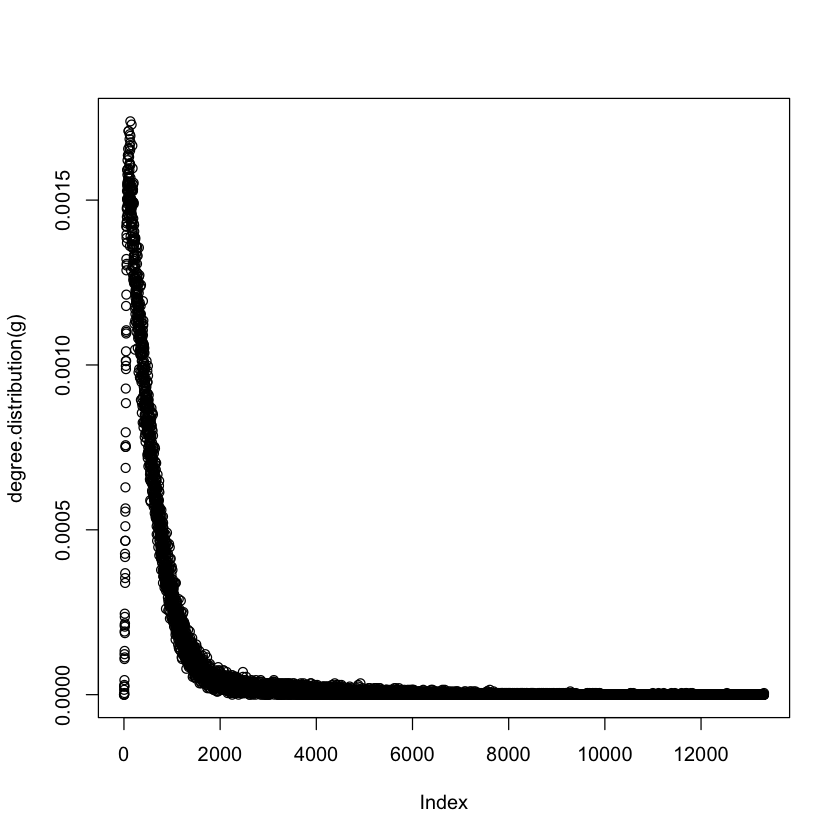
\includegraphics{Figures/F2_1.png}}
\caption{Degree distribution of the movie network}
\label{F2_1}
\end{figure}

\subsection{Communities in the movie network}
By detecting communities with Fast Greedy algorithm for our movie network, we got 28 communities. And for Quesition 7, we just picked the first 10 communities to plot the distribution of the genres of the movies in each community.

NOTICE: Some of the movies' genre information is missing in the given dataset, so we marked them as "NAN"; however, only Question 7, we considered them in our plots.

The 10 plots are shown in Figure \ref{fig:Q7_1} to Figure \ref{fig:Q7_10}.

\begin{figure}[H]
\centering
\scalebox{1}{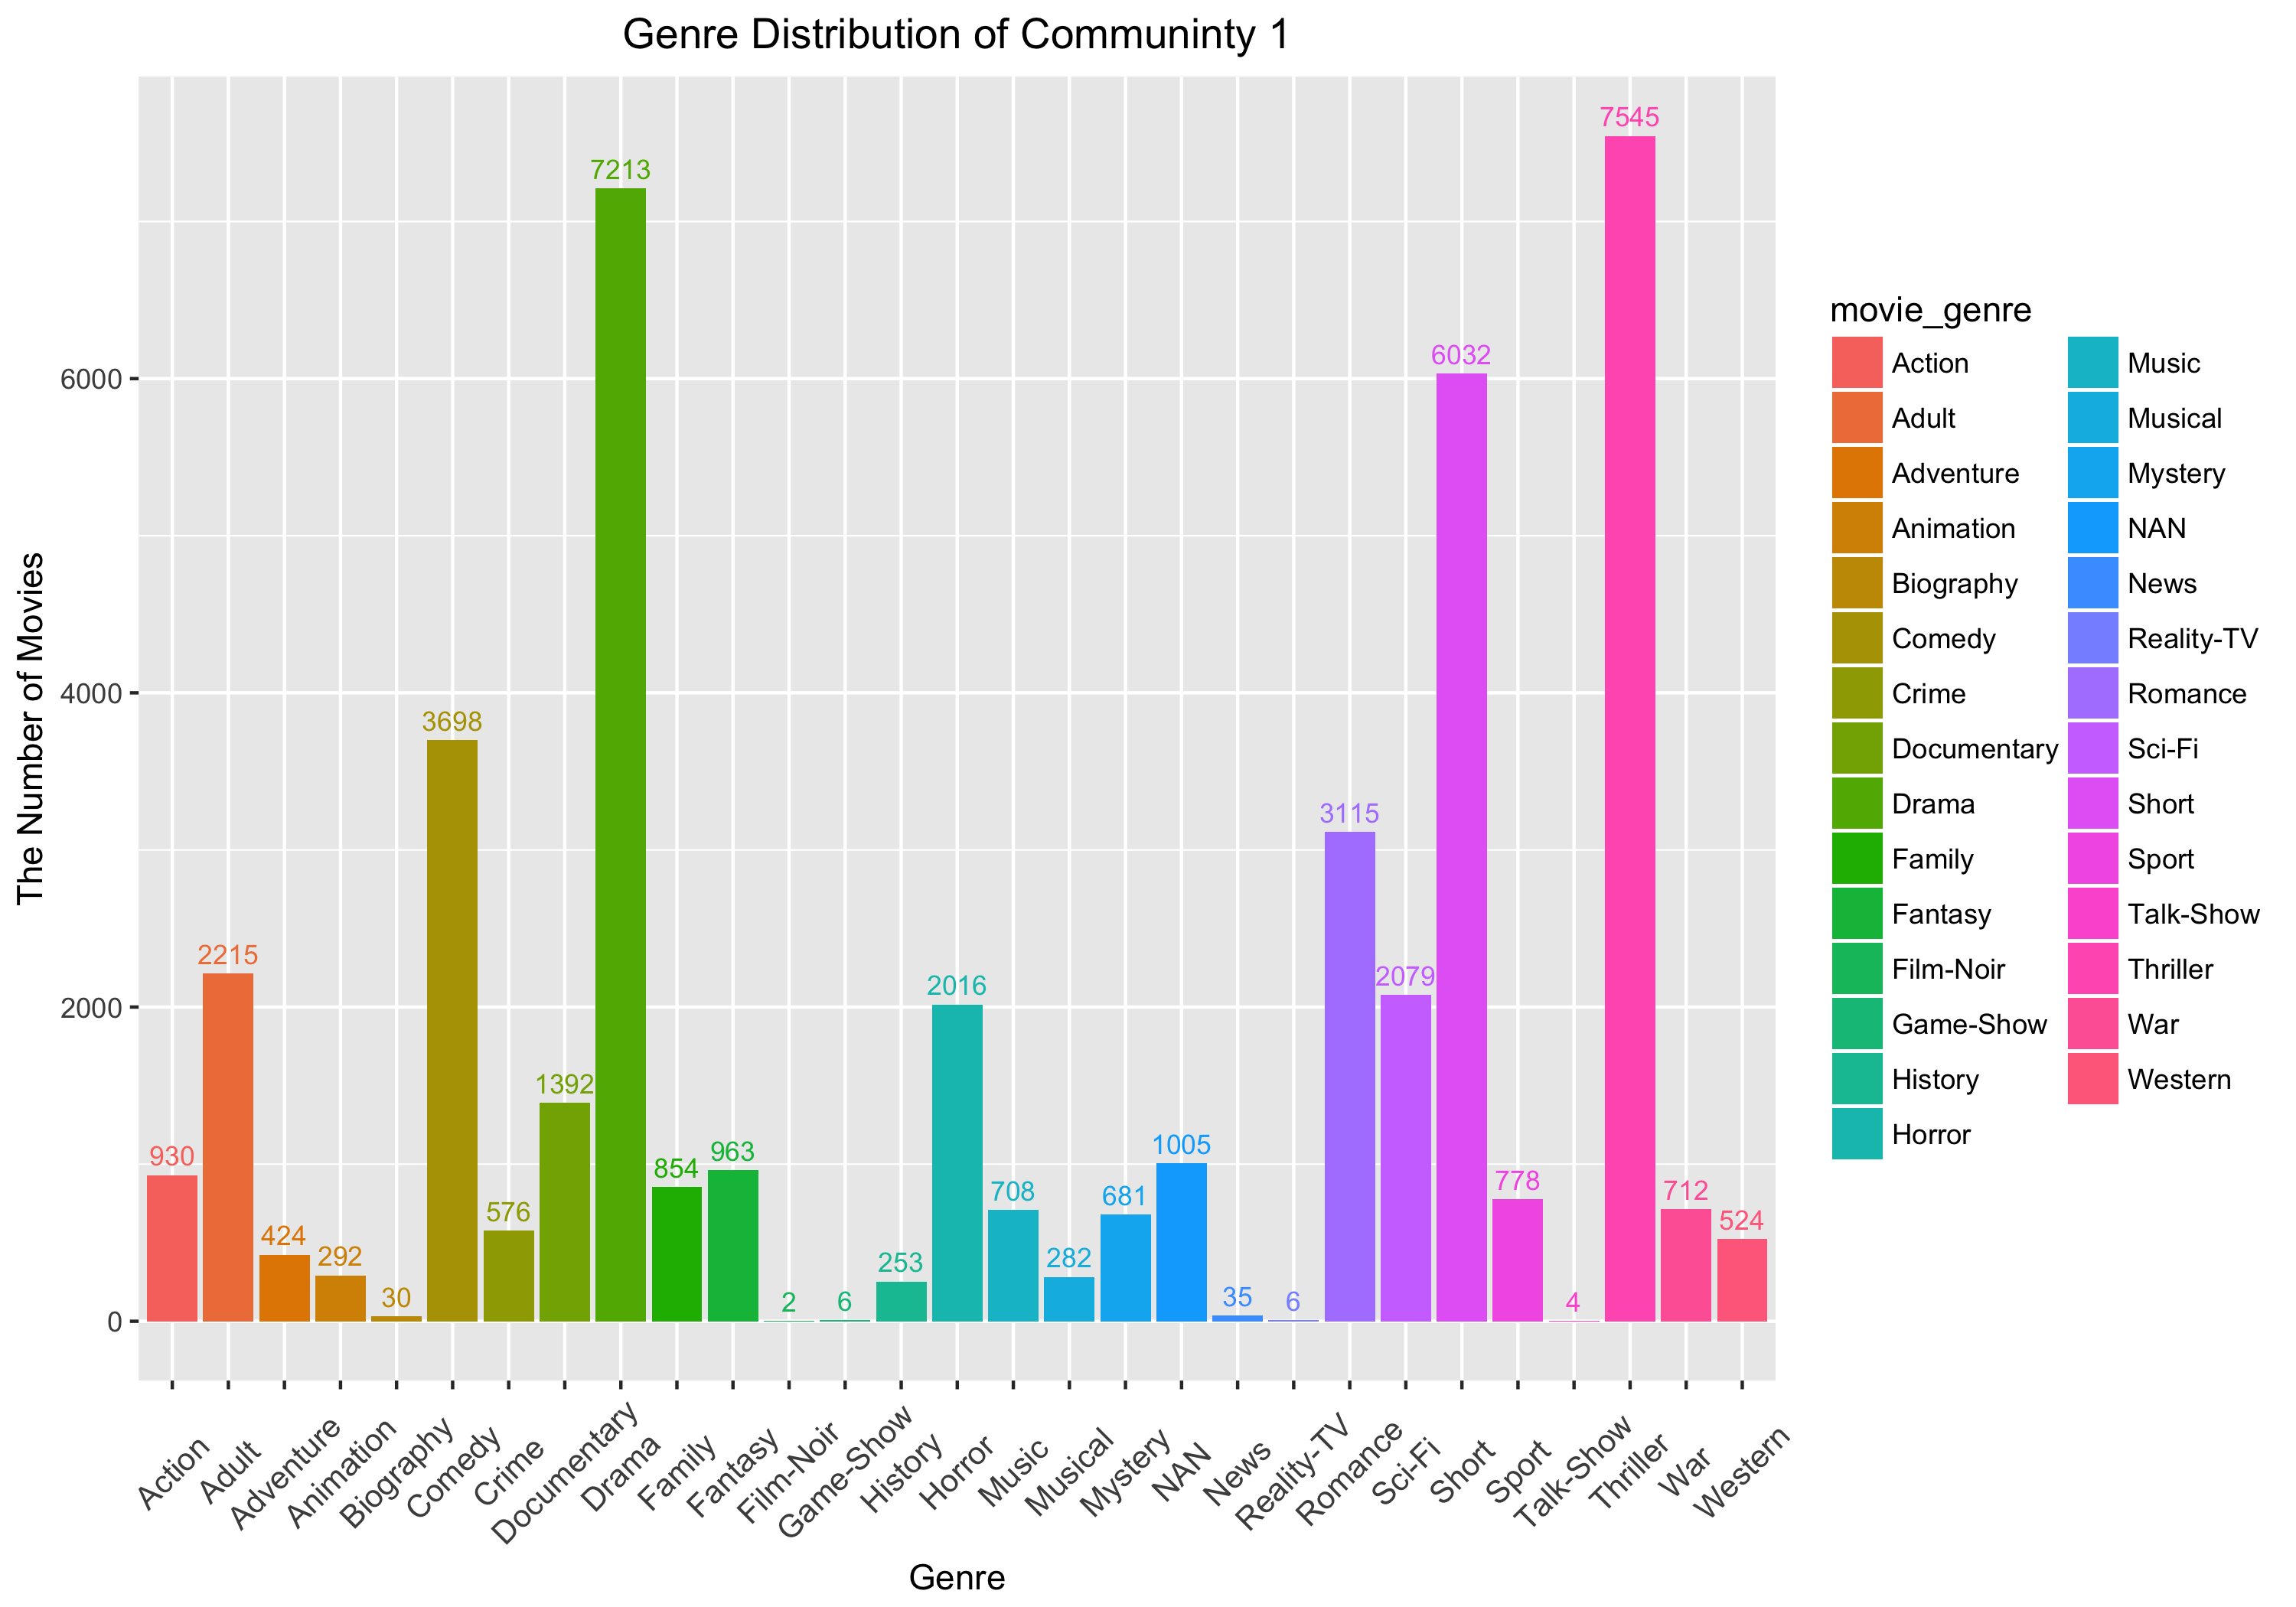
\includegraphics{Figures/community_1.png}}
\caption{Genre Distribution of Community $1$}
\label{fig:Q7_1}
\end{figure}

\begin{figure}[H]
\centering
\scalebox{1}{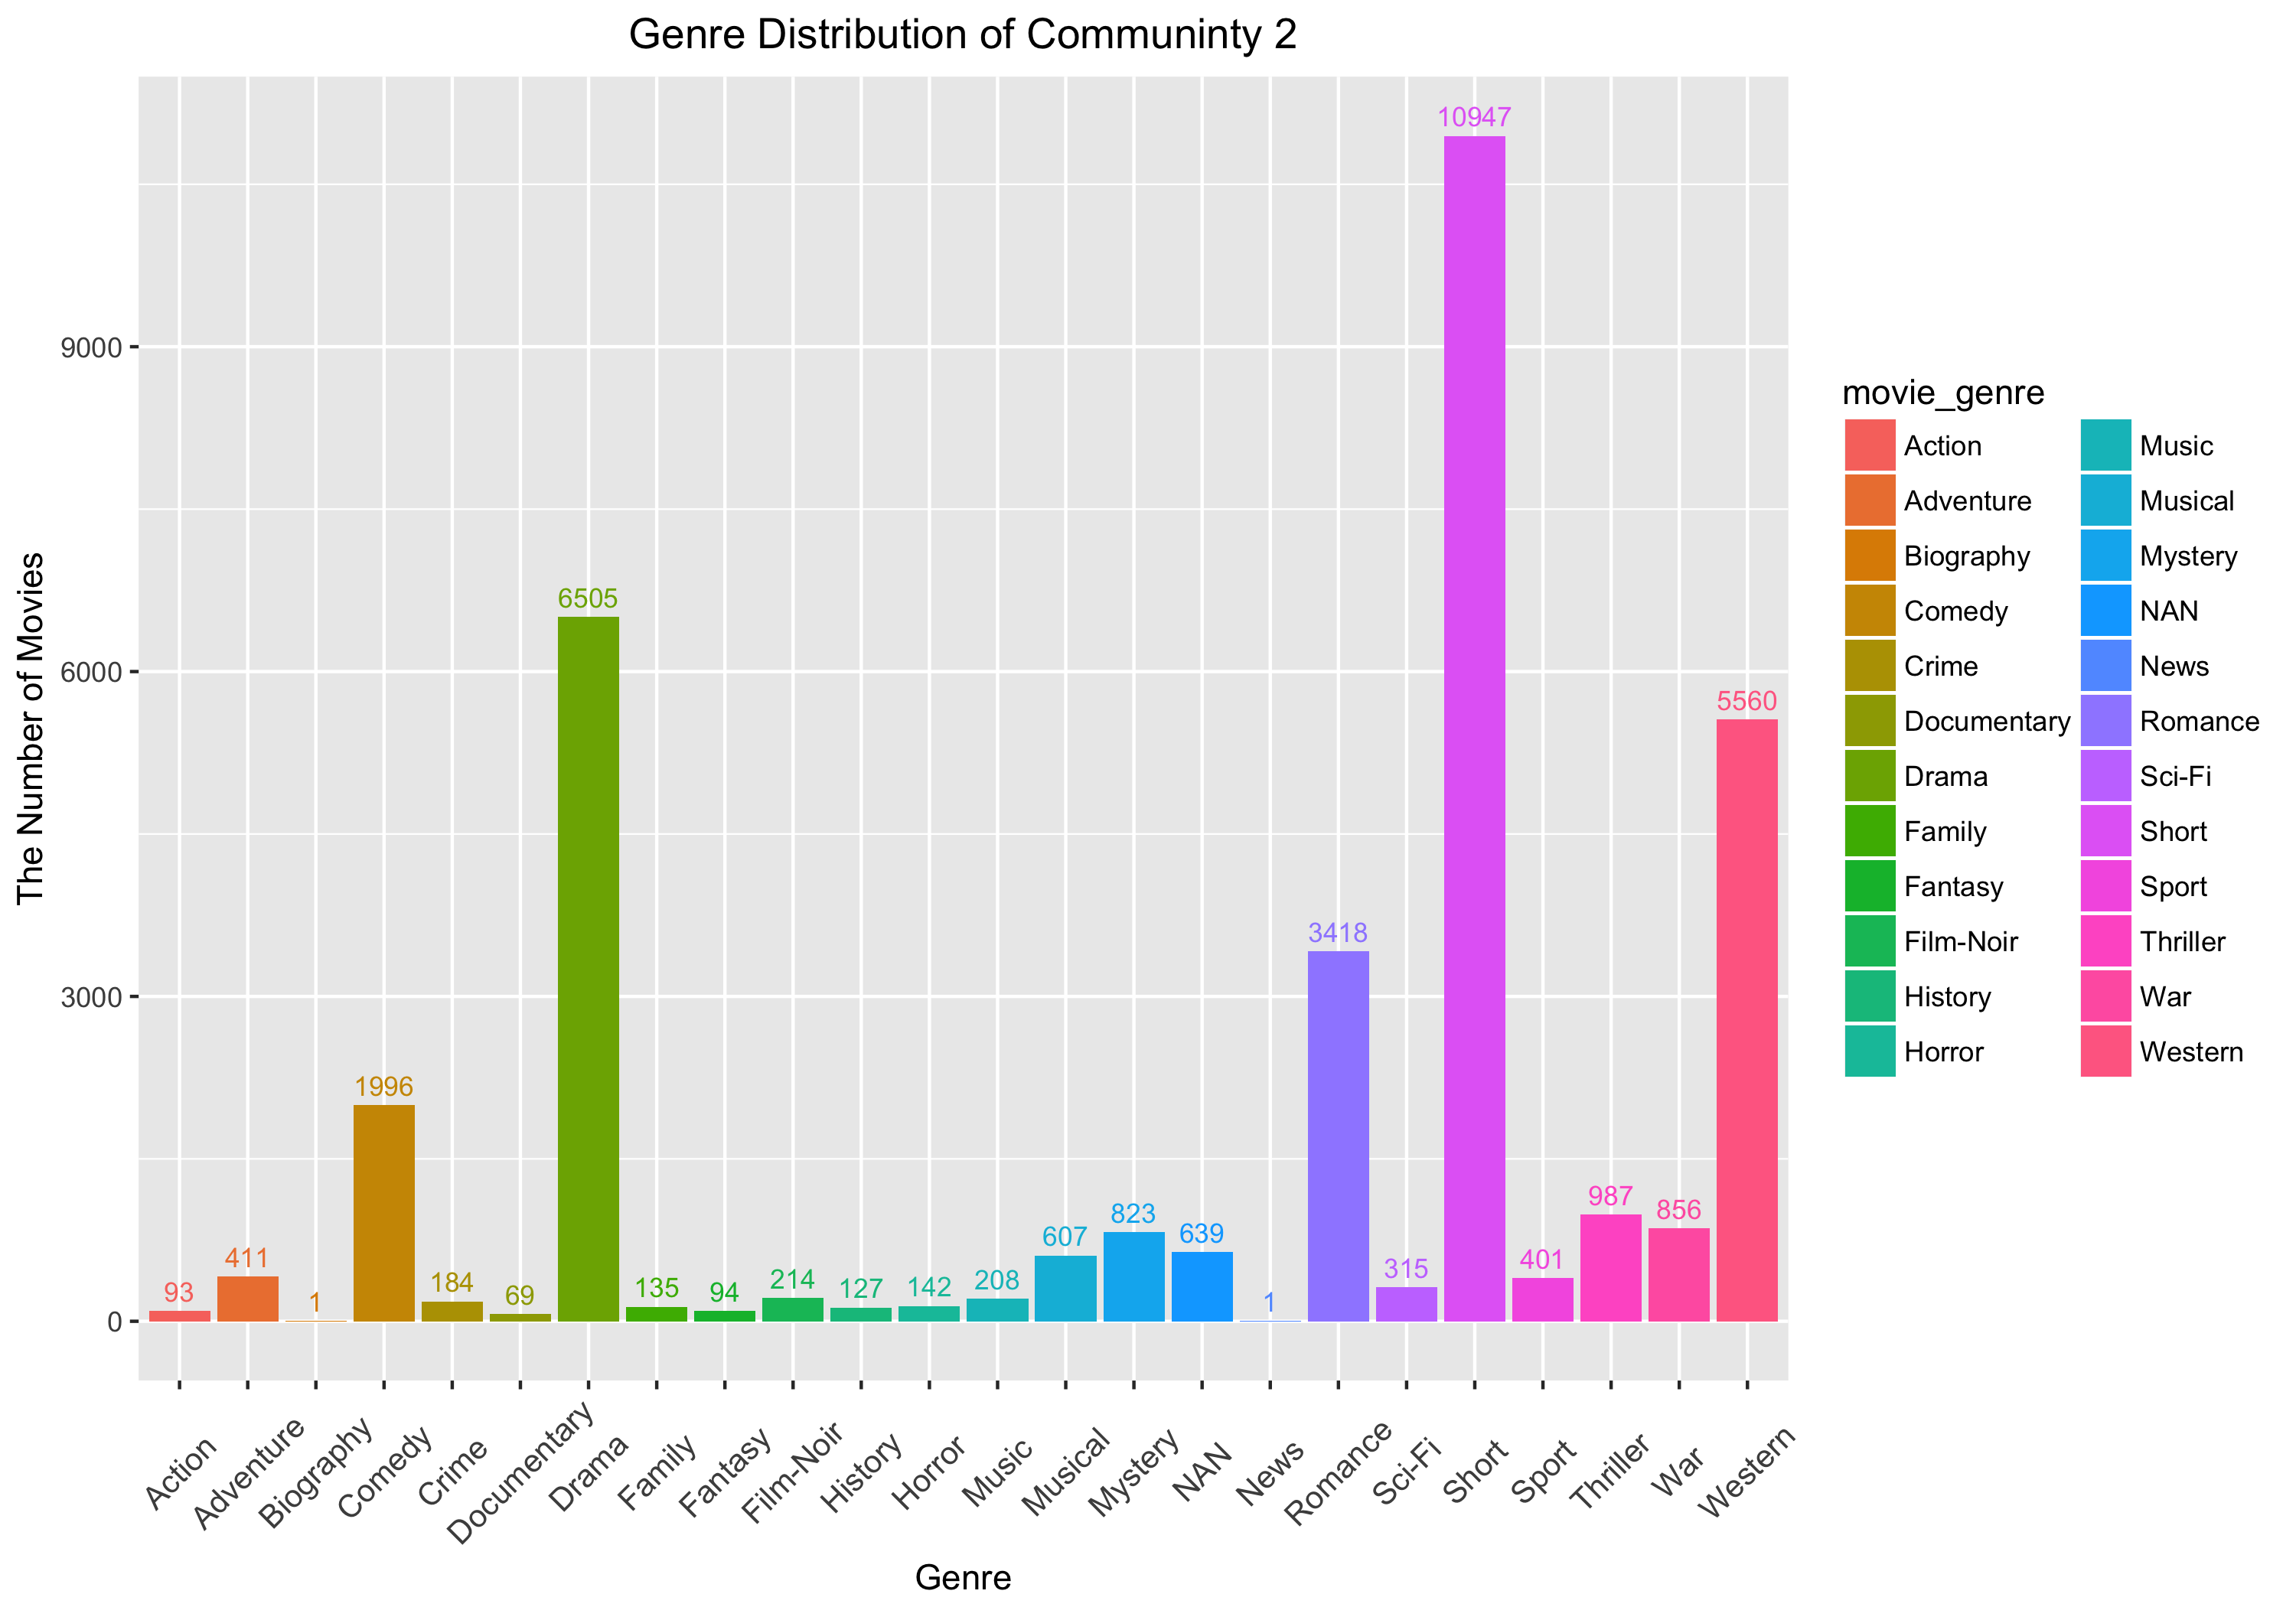
\includegraphics{Figures/community_2.png}}
\caption{Genre Distribution of Community $2$}
\label{fig:Q7_2}
\end{figure}

\begin{figure}[H]
\centering
\scalebox{1}{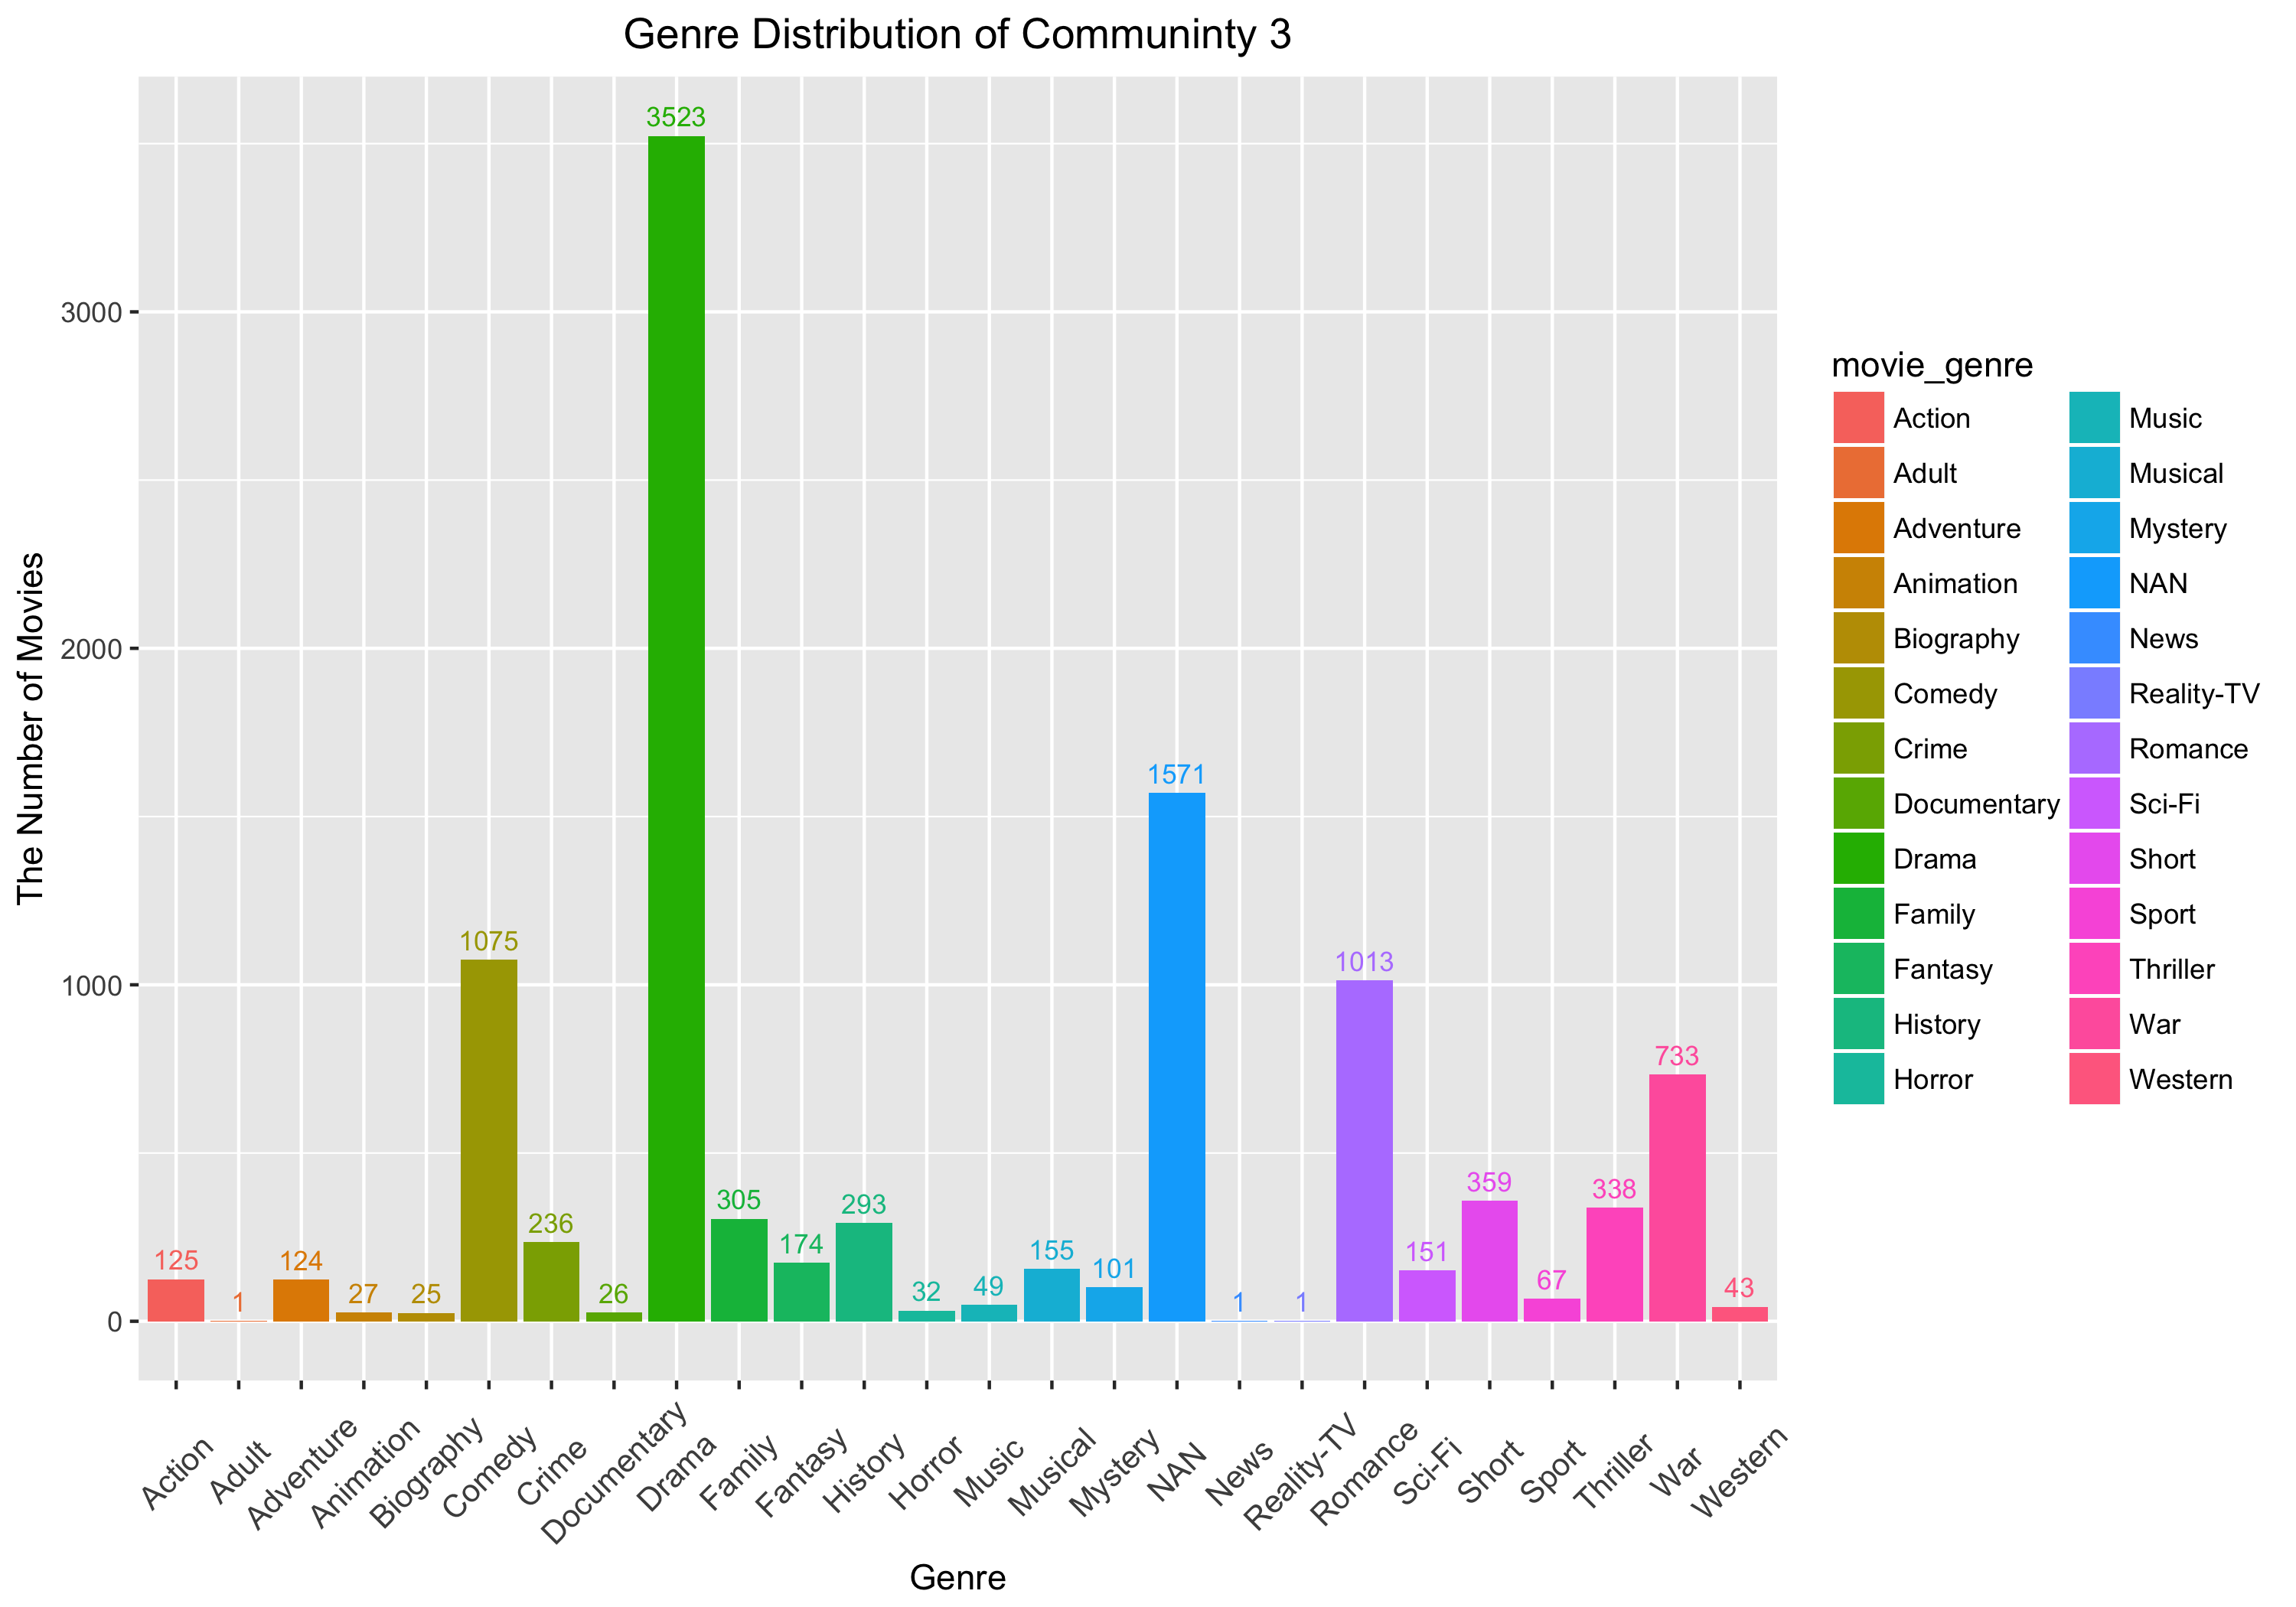
\includegraphics{Figures/community_3.png}}
\caption{Genre Distribution of Community $3$}
\label{fig:Q7_3}
\end{figure}

\begin{figure}[H]
\centering
\scalebox{1}{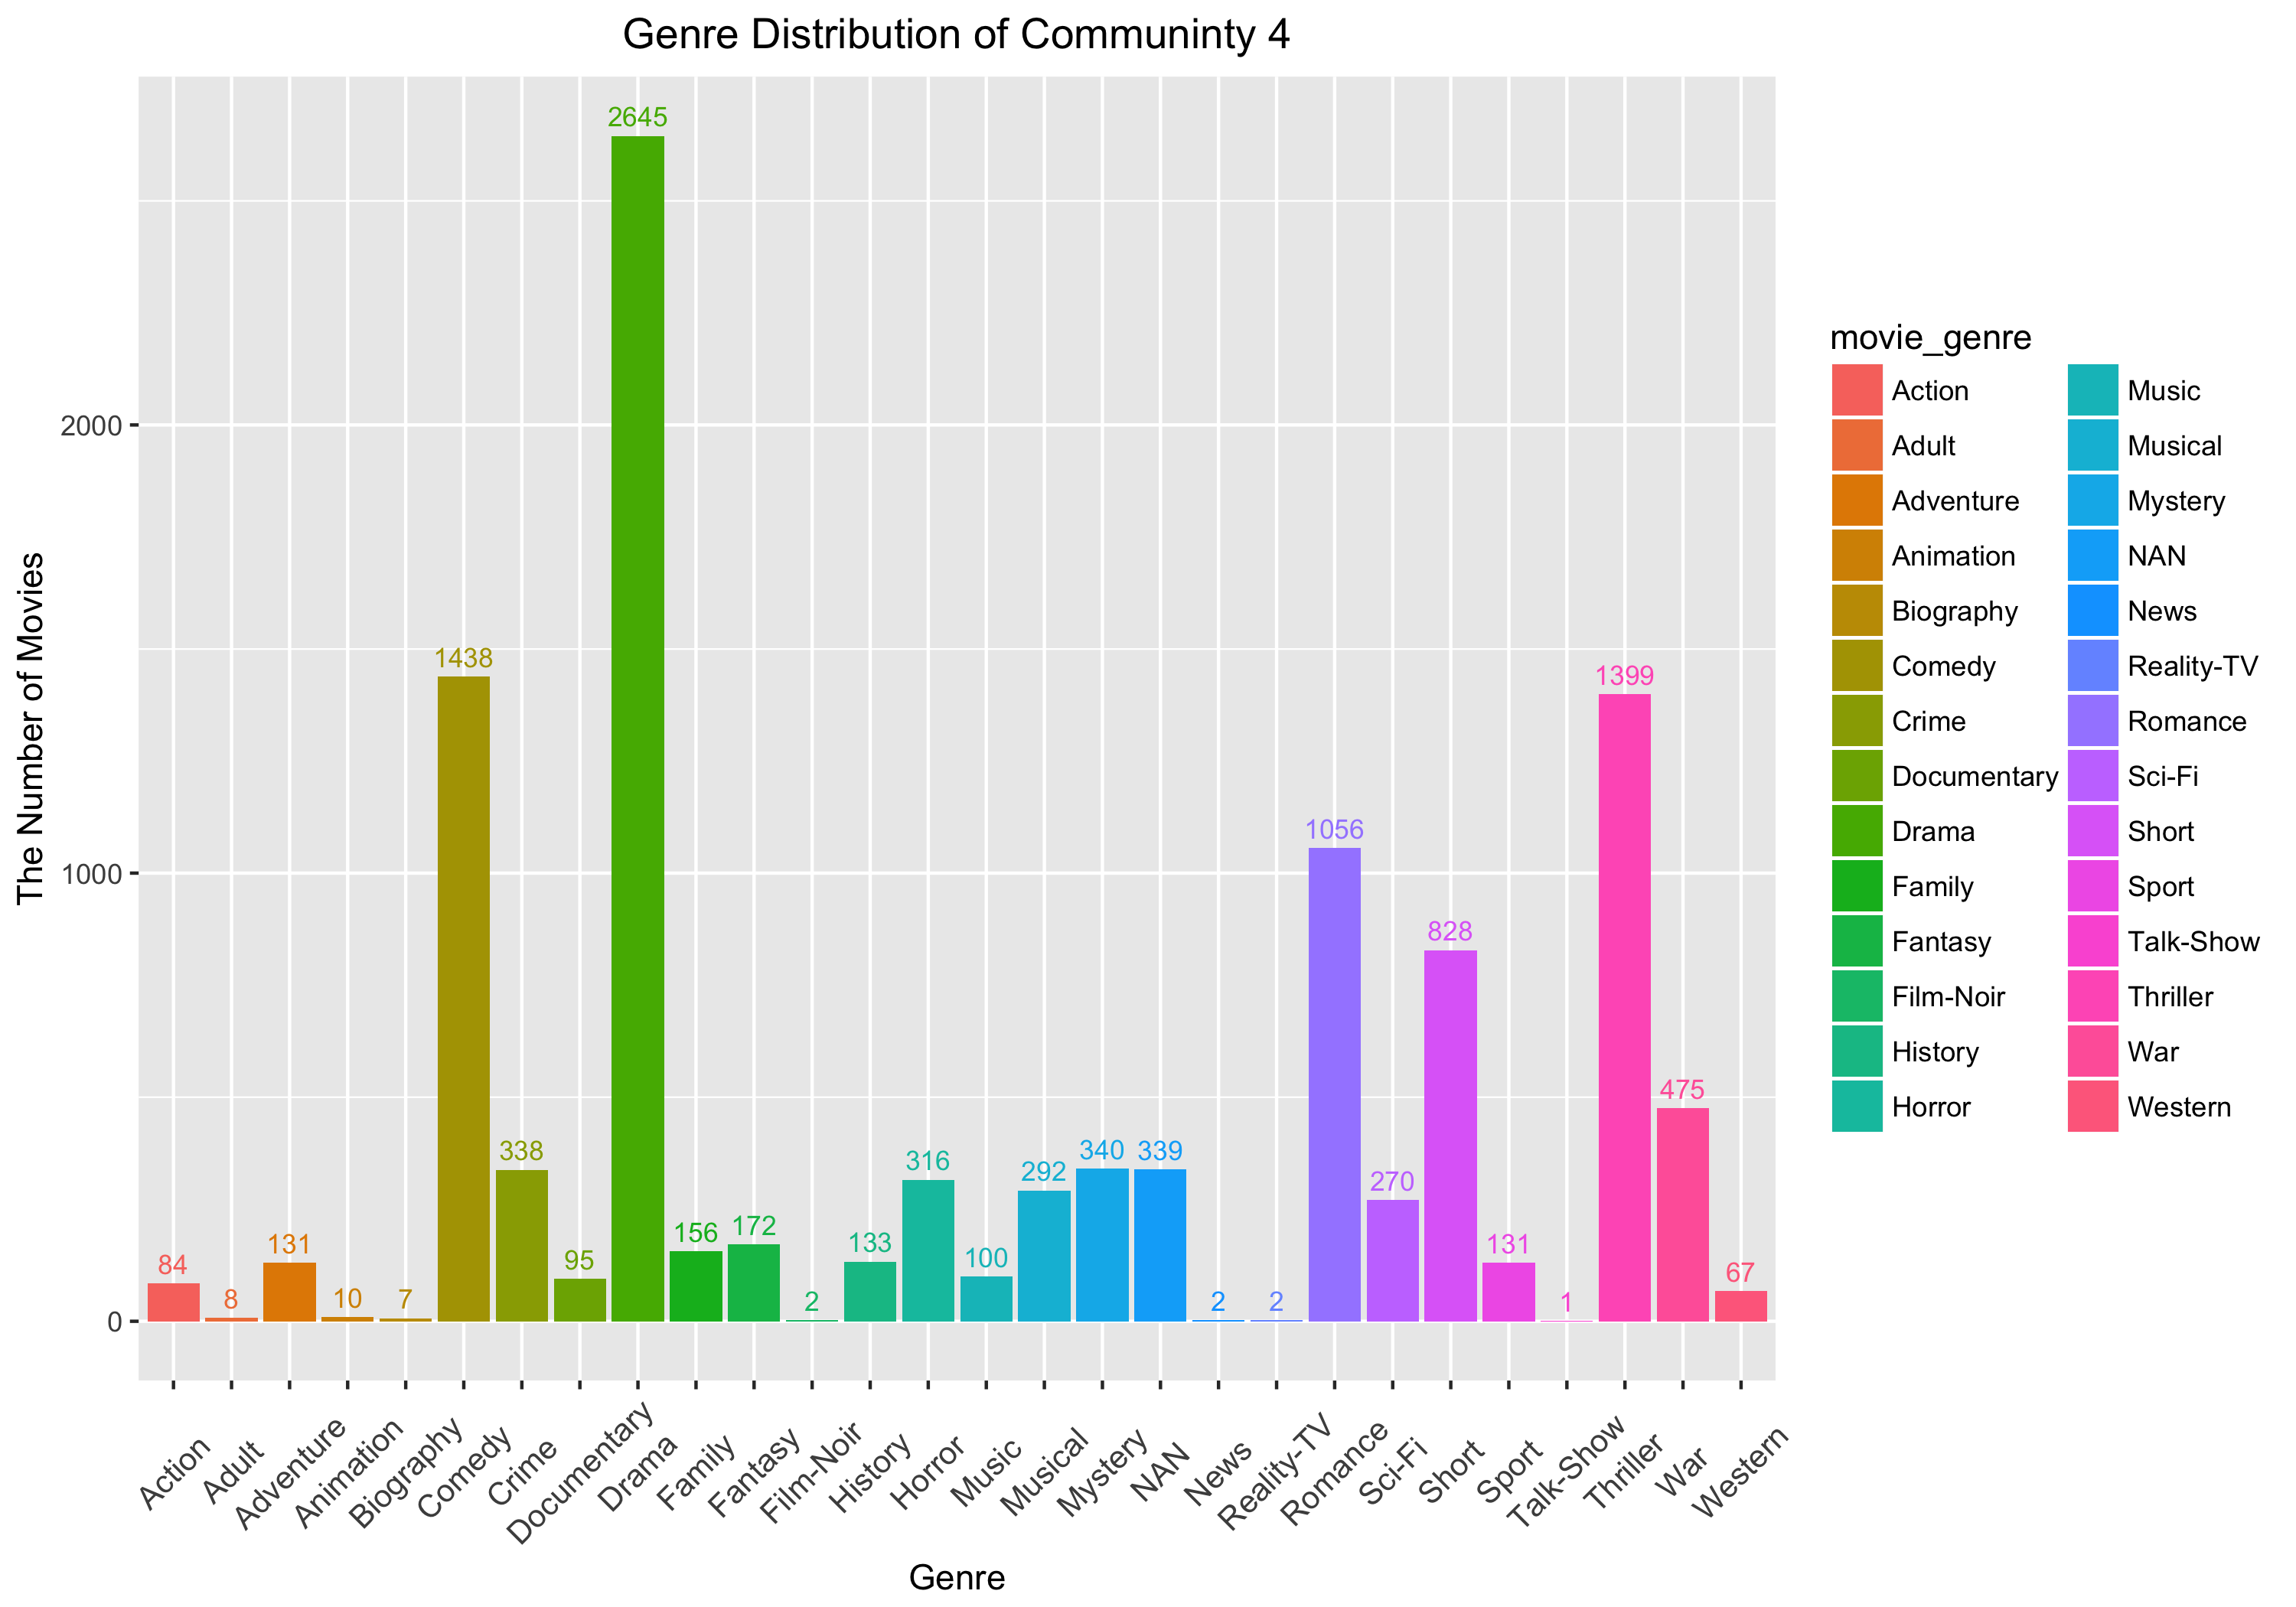
\includegraphics{Figures/community_4.png}}
\caption{Genre Distribution of Community $4$}
\label{fig:Q7_4}
\end{figure}

\begin{figure}[H]
\centering
\scalebox{1}{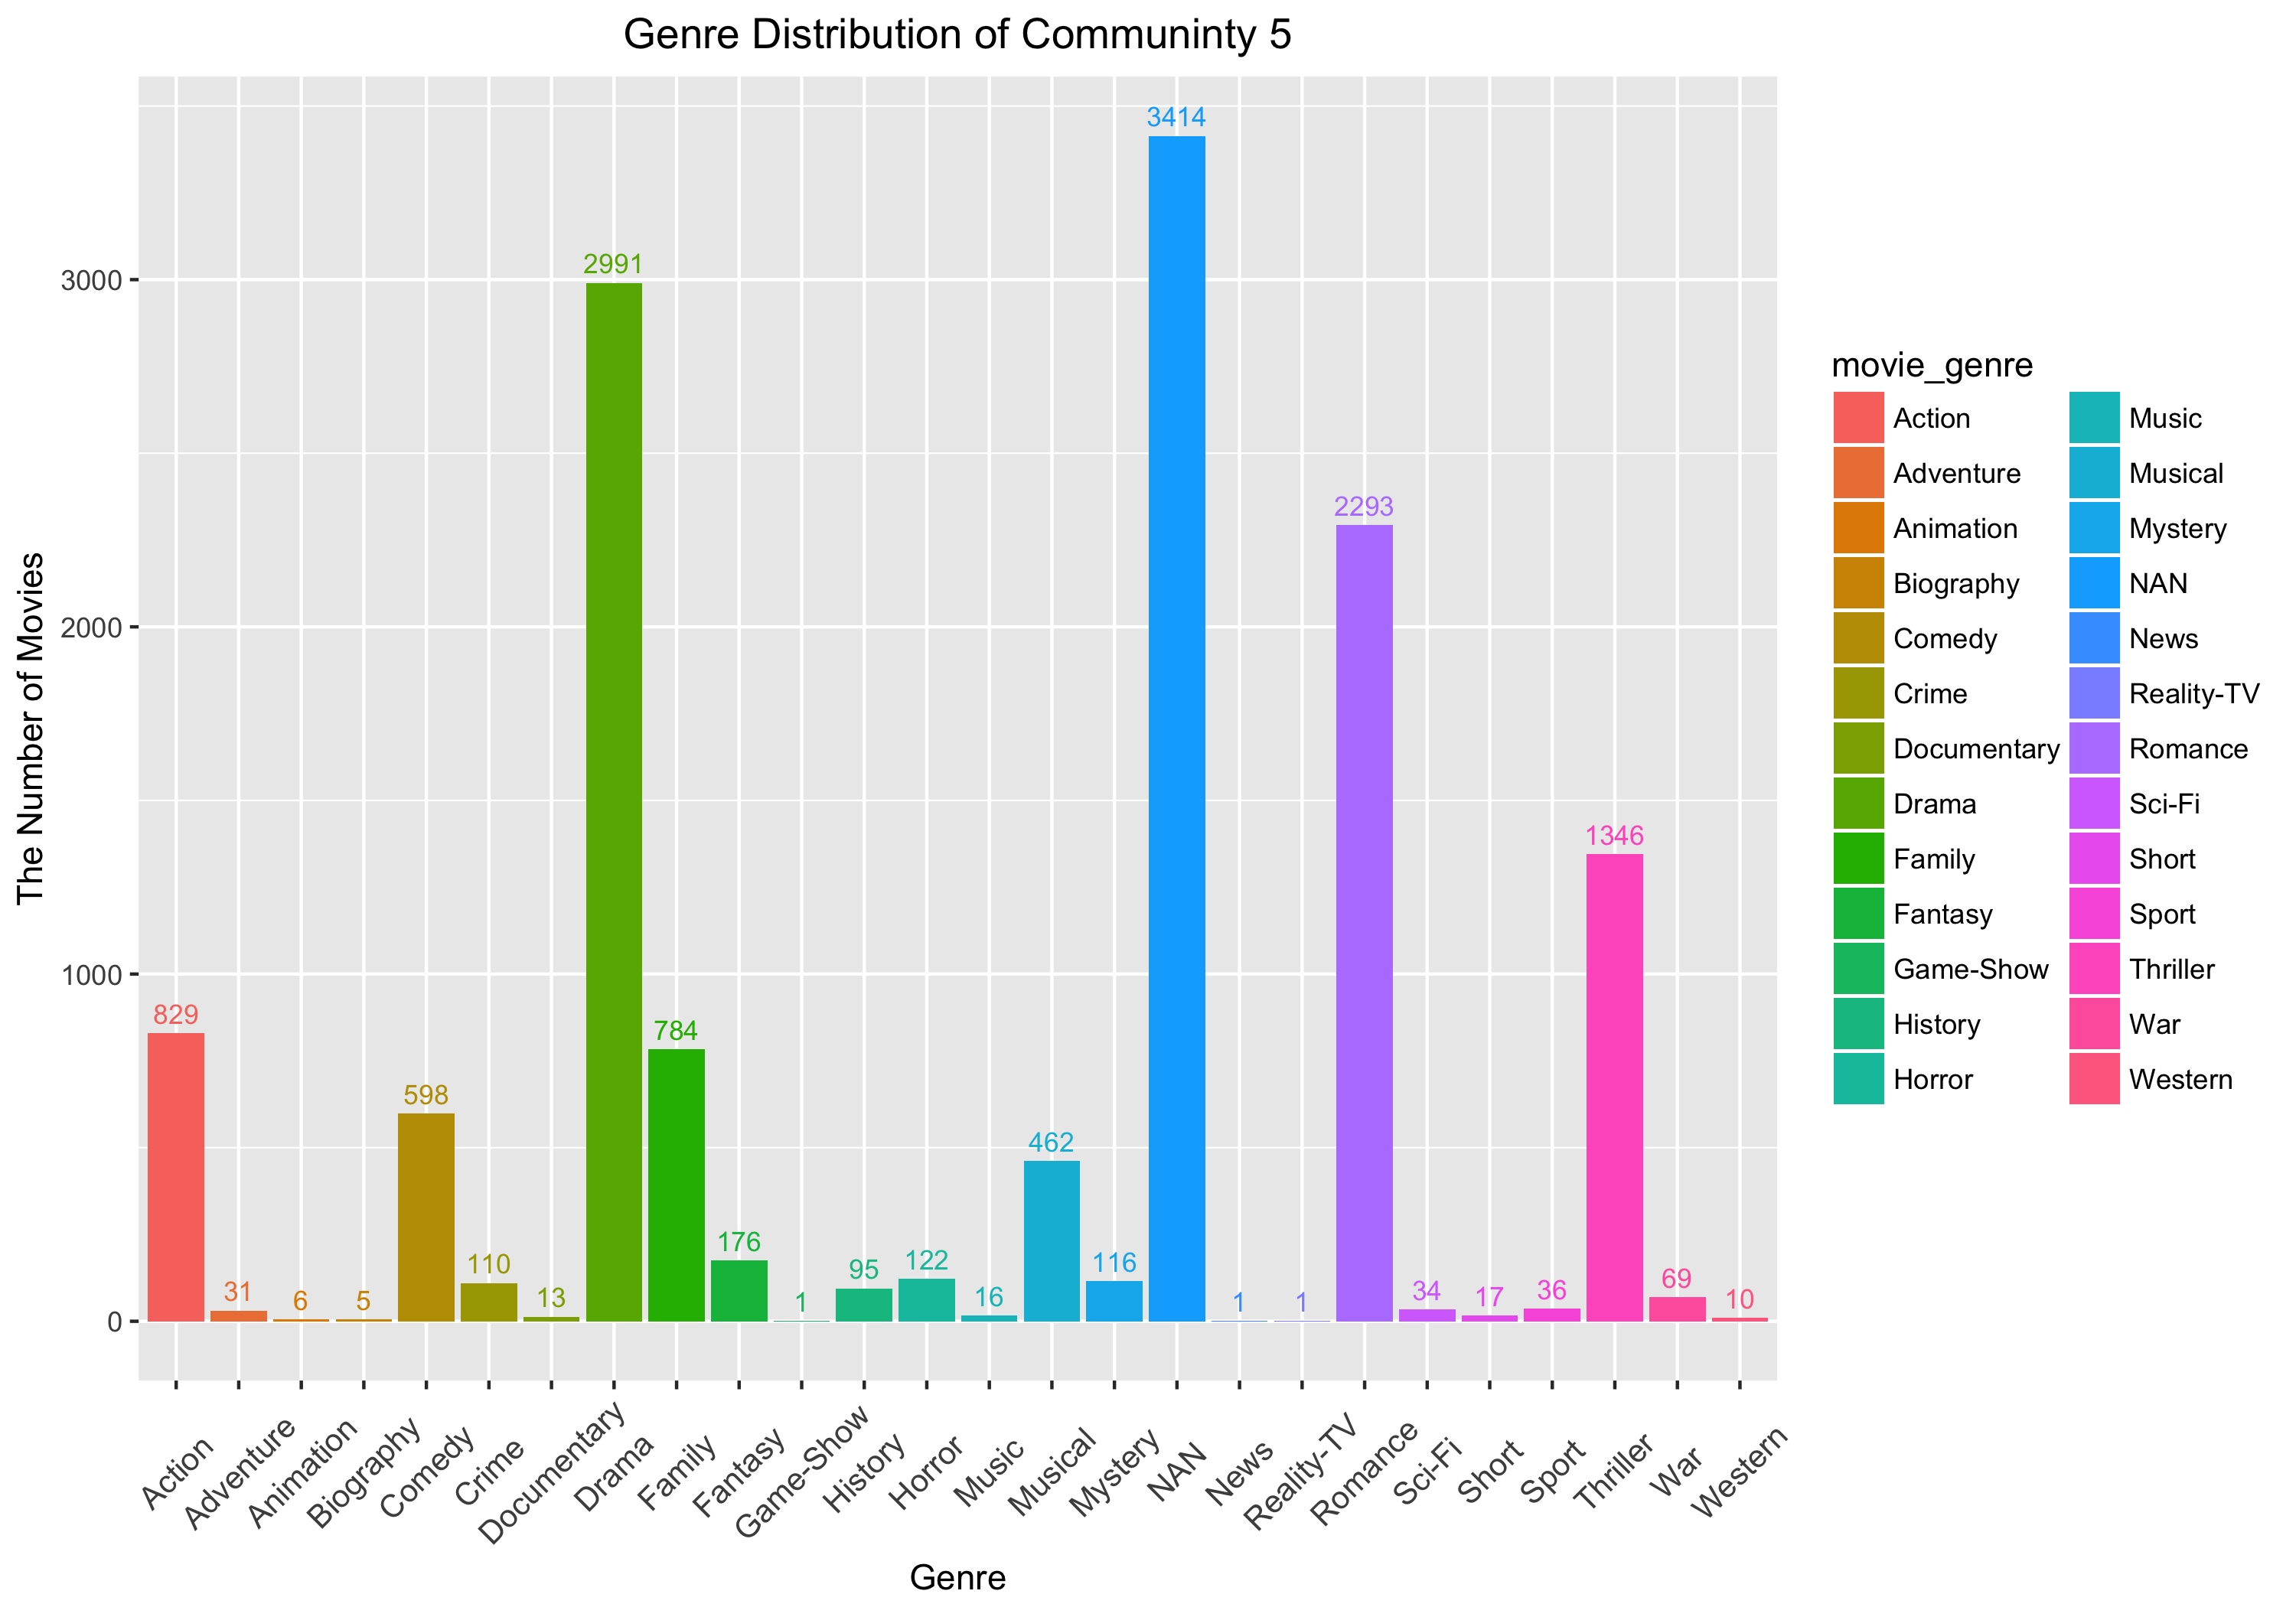
\includegraphics{Figures/community_5.png}}
\caption{Genre Distribution of Community $5$}
\label{fig:Q7_5}
\end{figure}

\begin{figure}[H]
\centering
\scalebox{1}{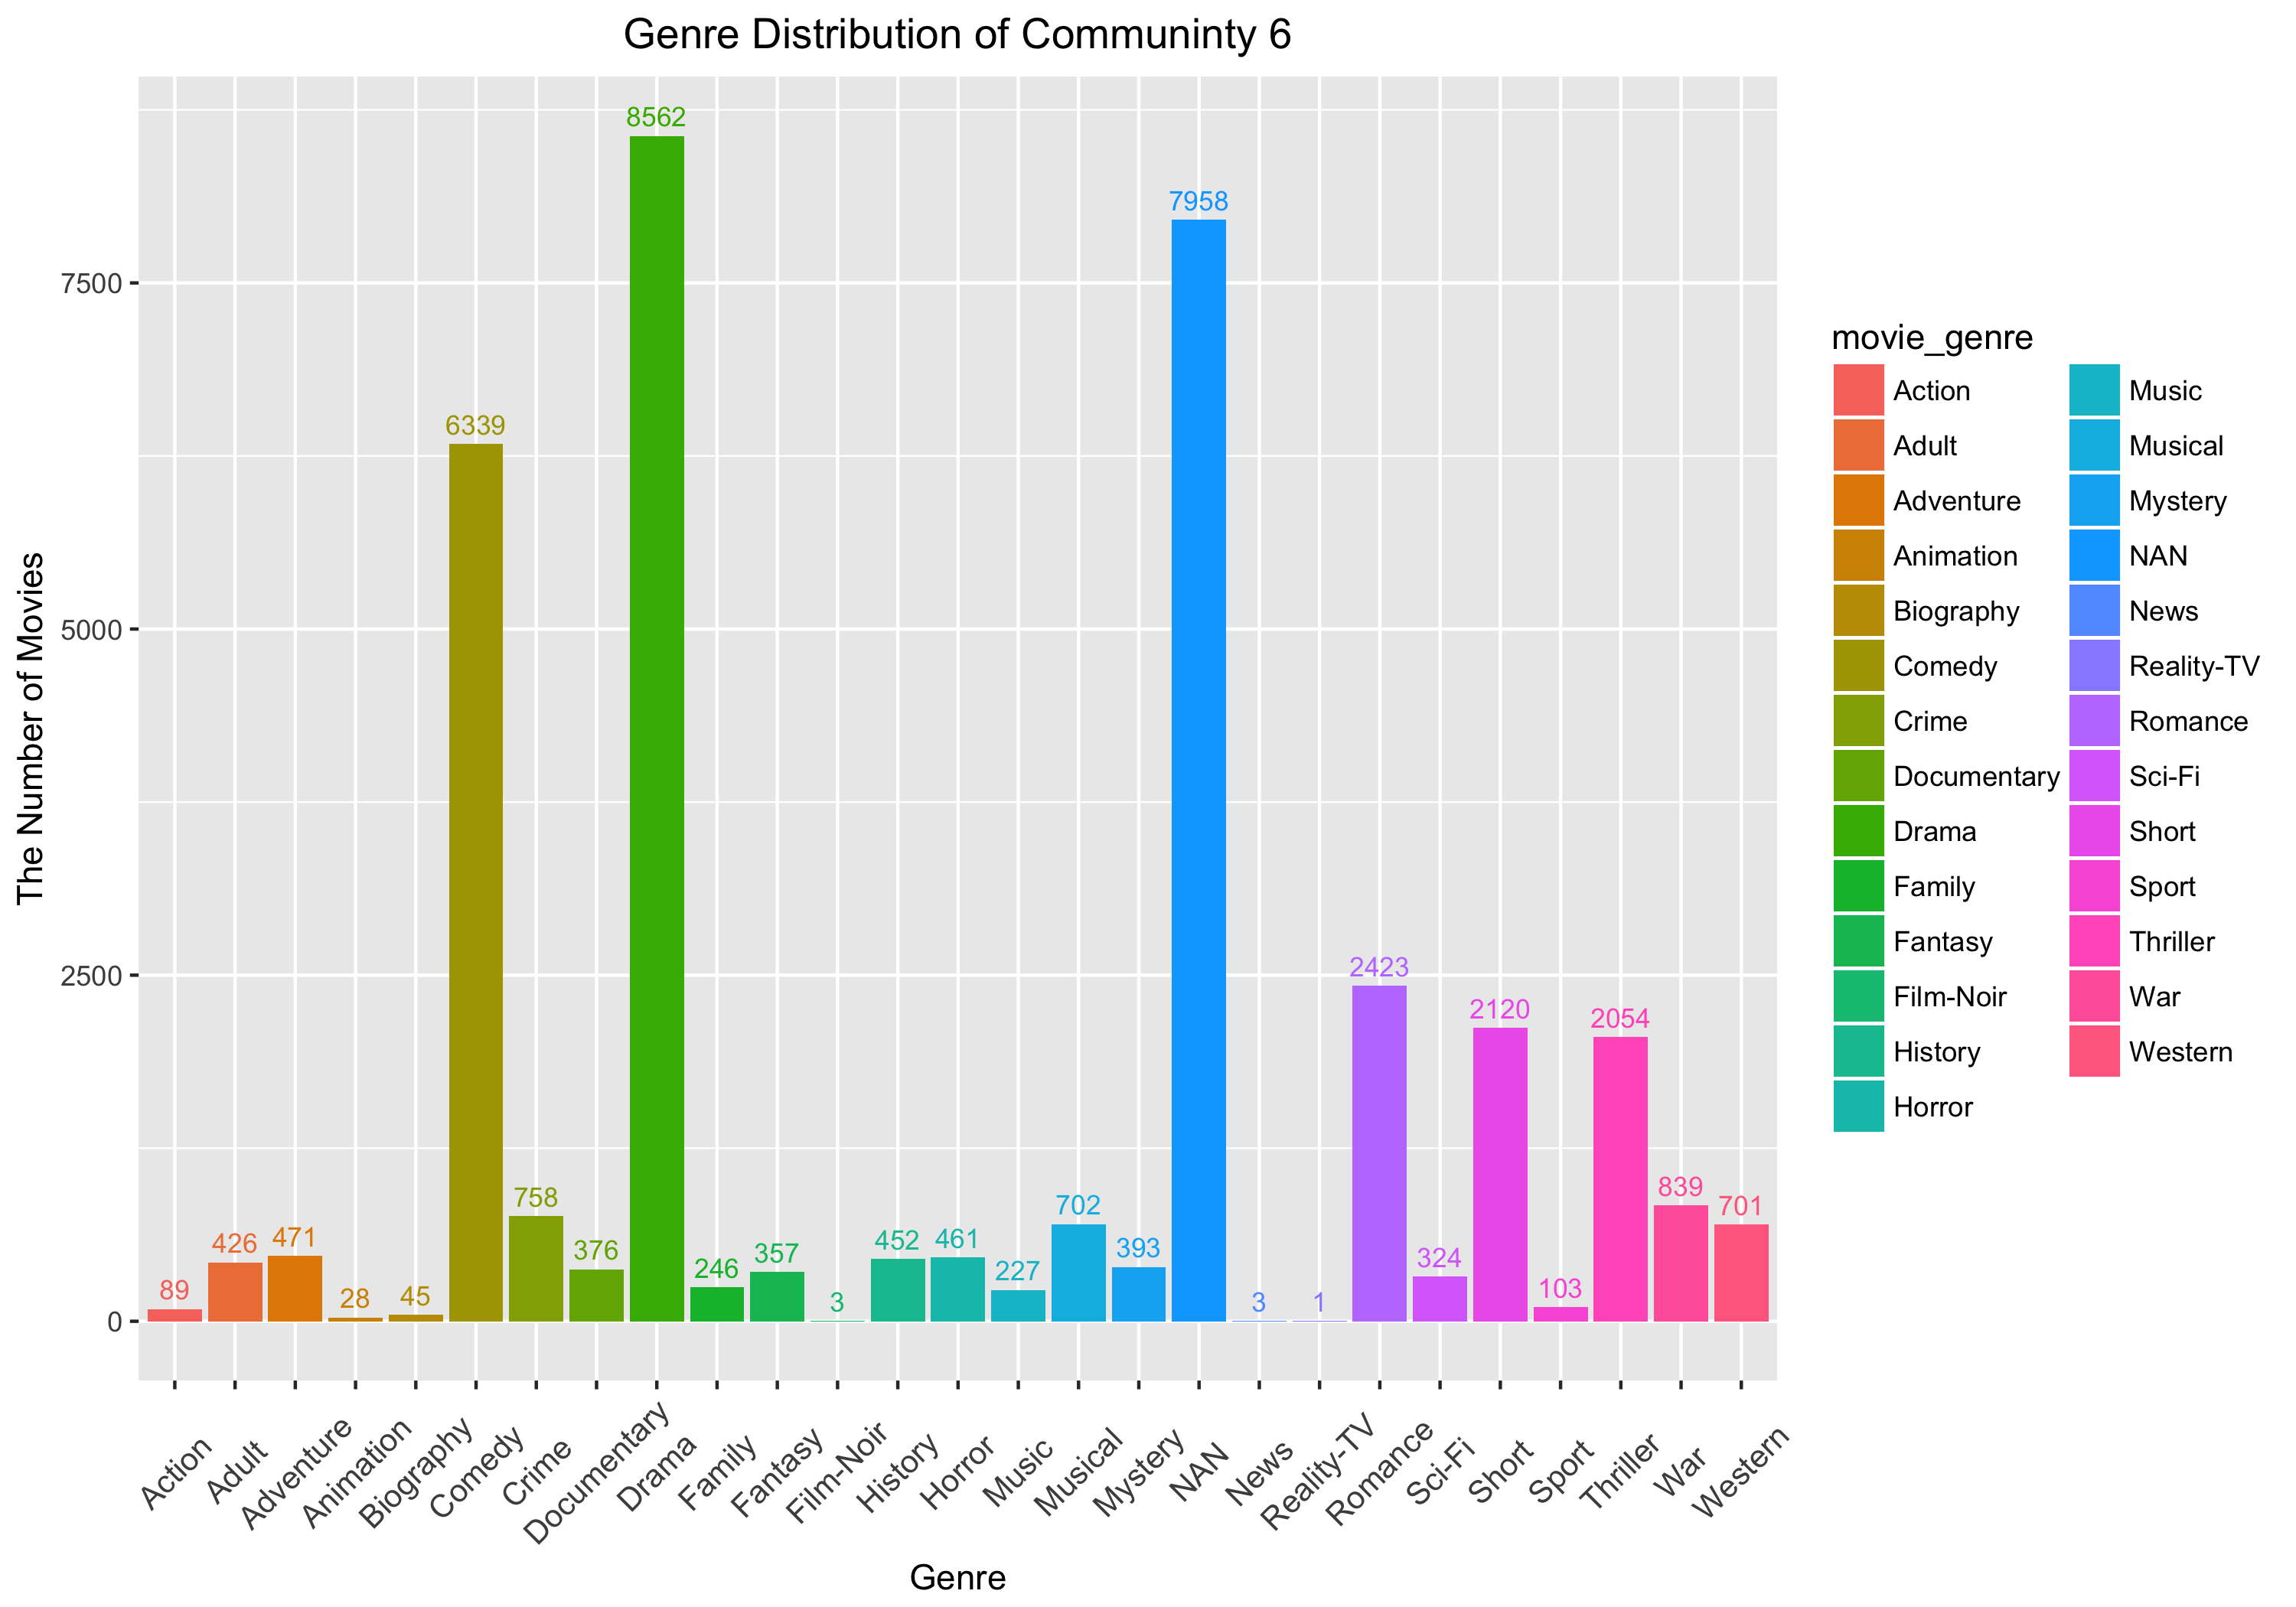
\includegraphics{Figures/community_6.png}}
\caption{Genre Distribution of Community $6$}
\label{fig:Q7_6}
\end{figure}

\begin{figure}[H]
\centering
\scalebox{1}{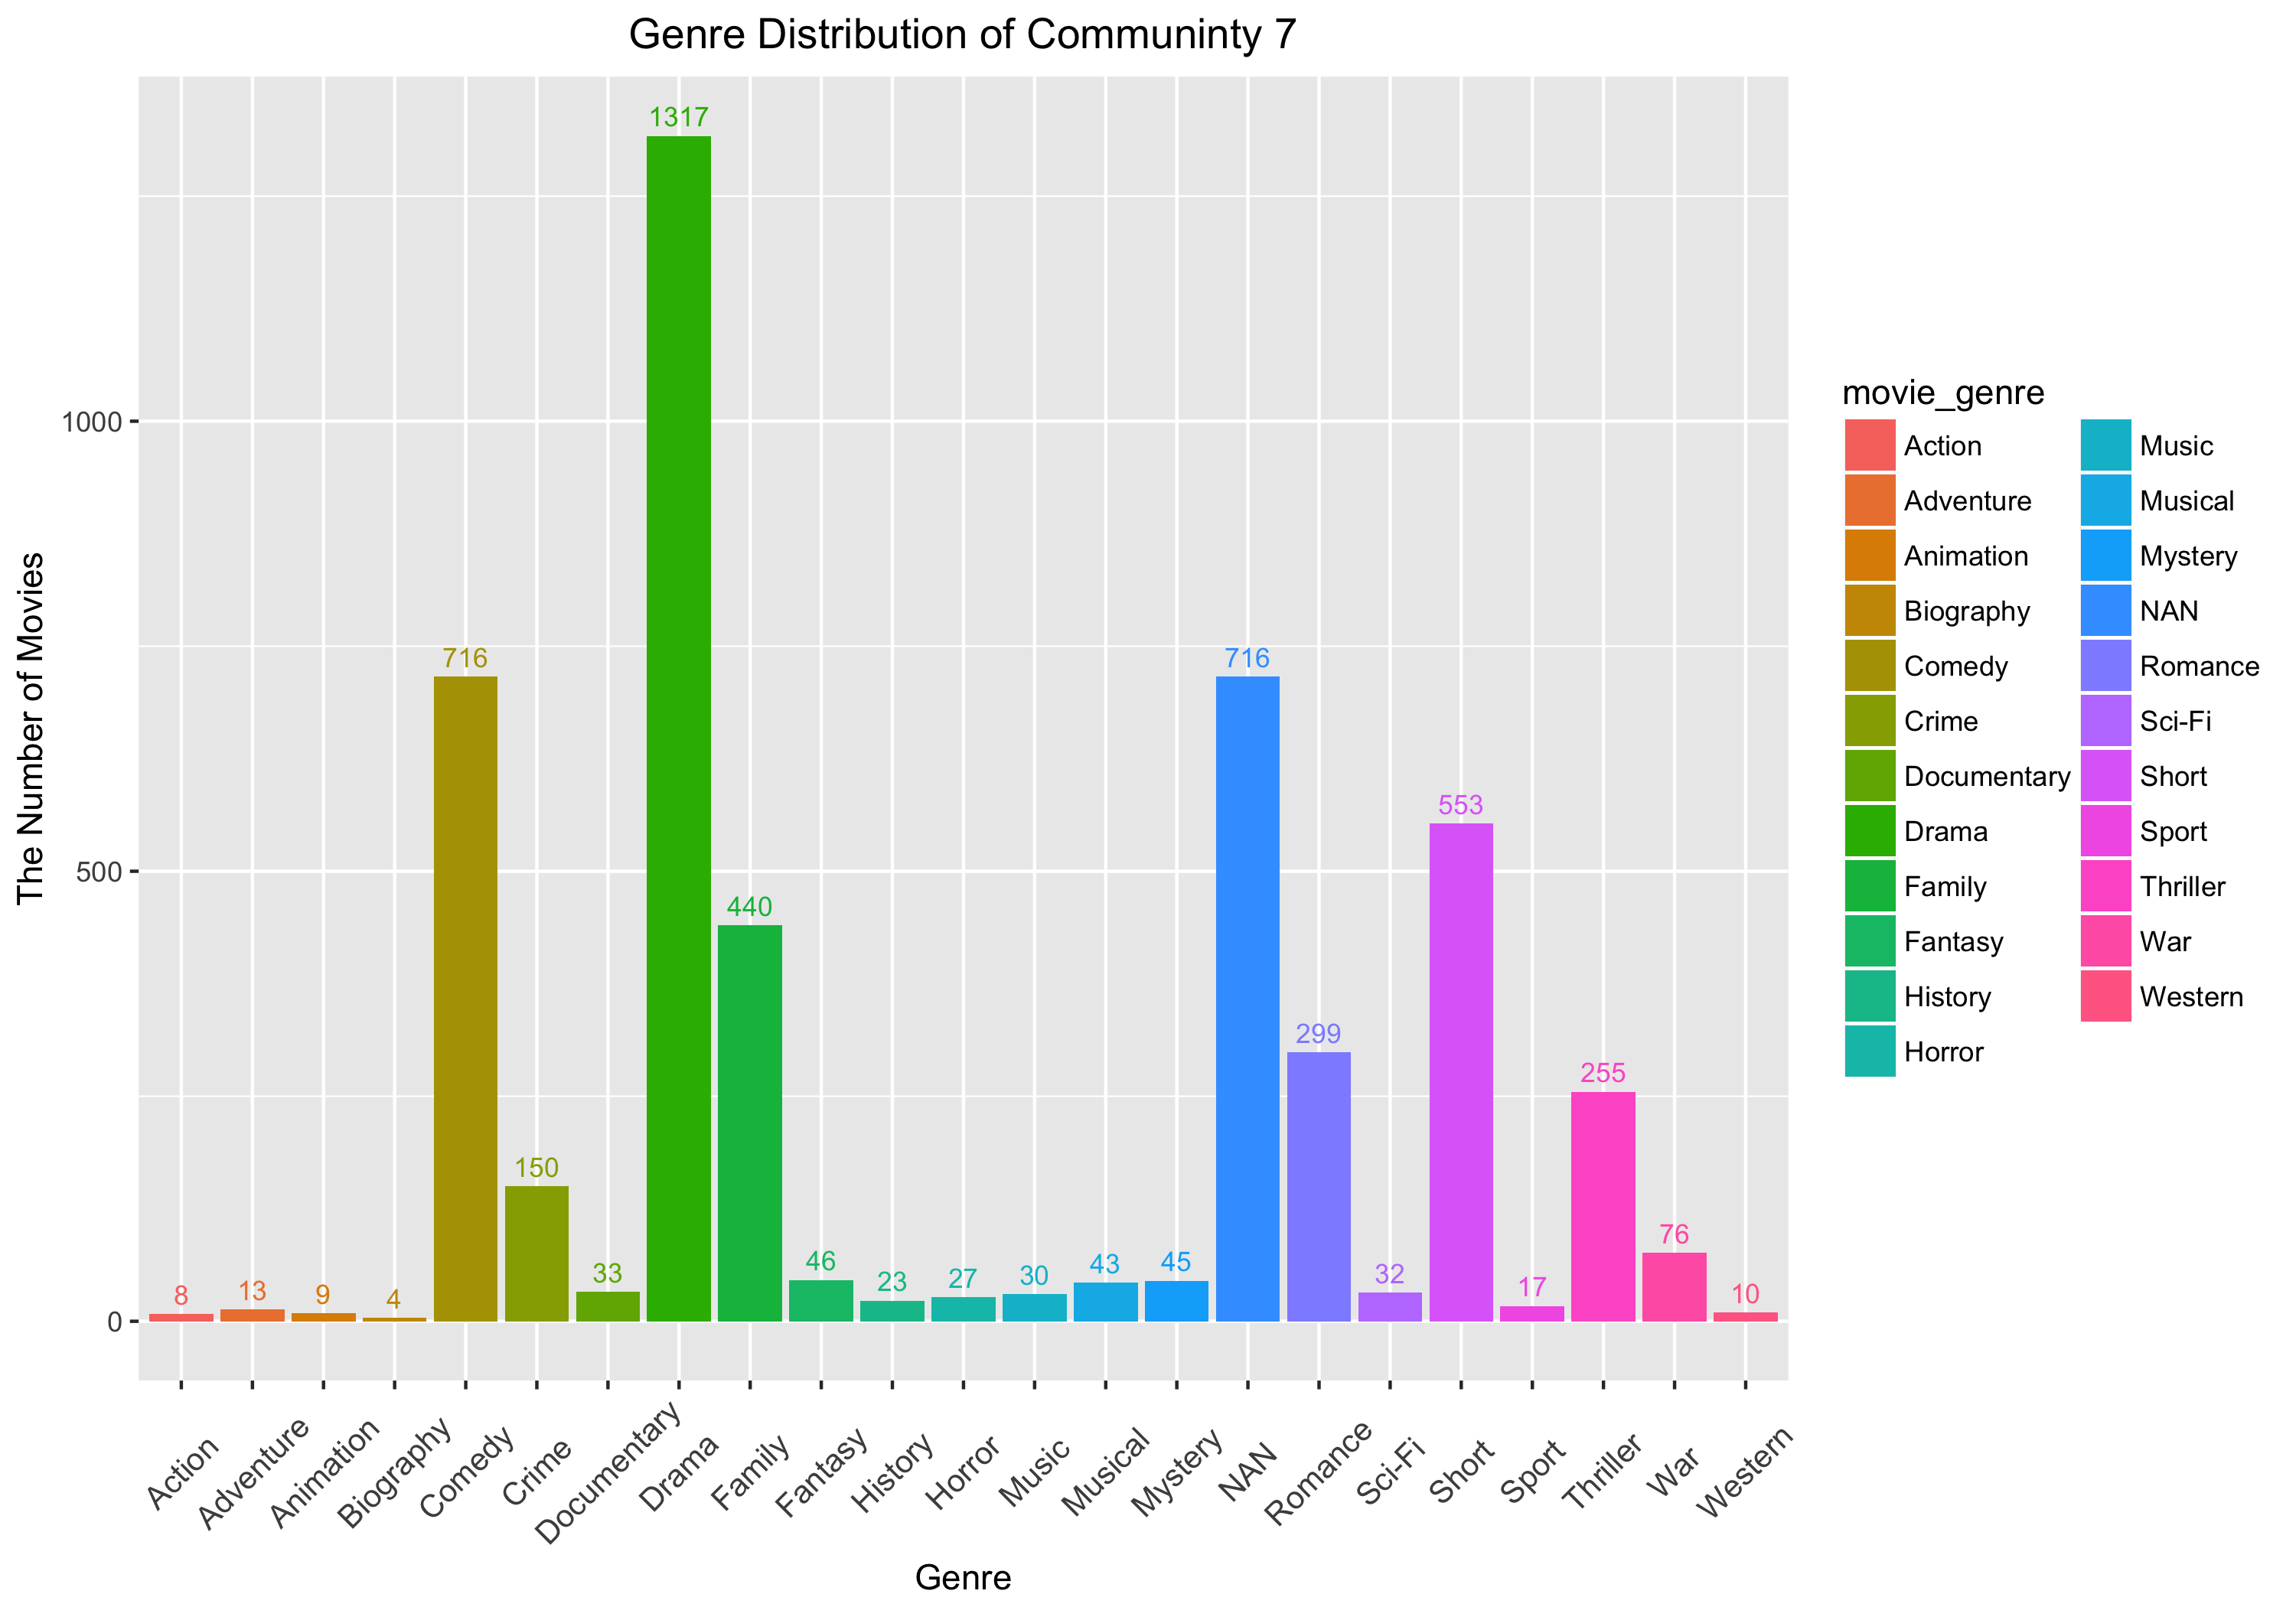
\includegraphics{Figures/community_7.png}}
\caption{Genre Distribution of Community $7$}
\label{fig:Q7_7}
\end{figure}

\begin{figure}[H]
\centering
\scalebox{1}{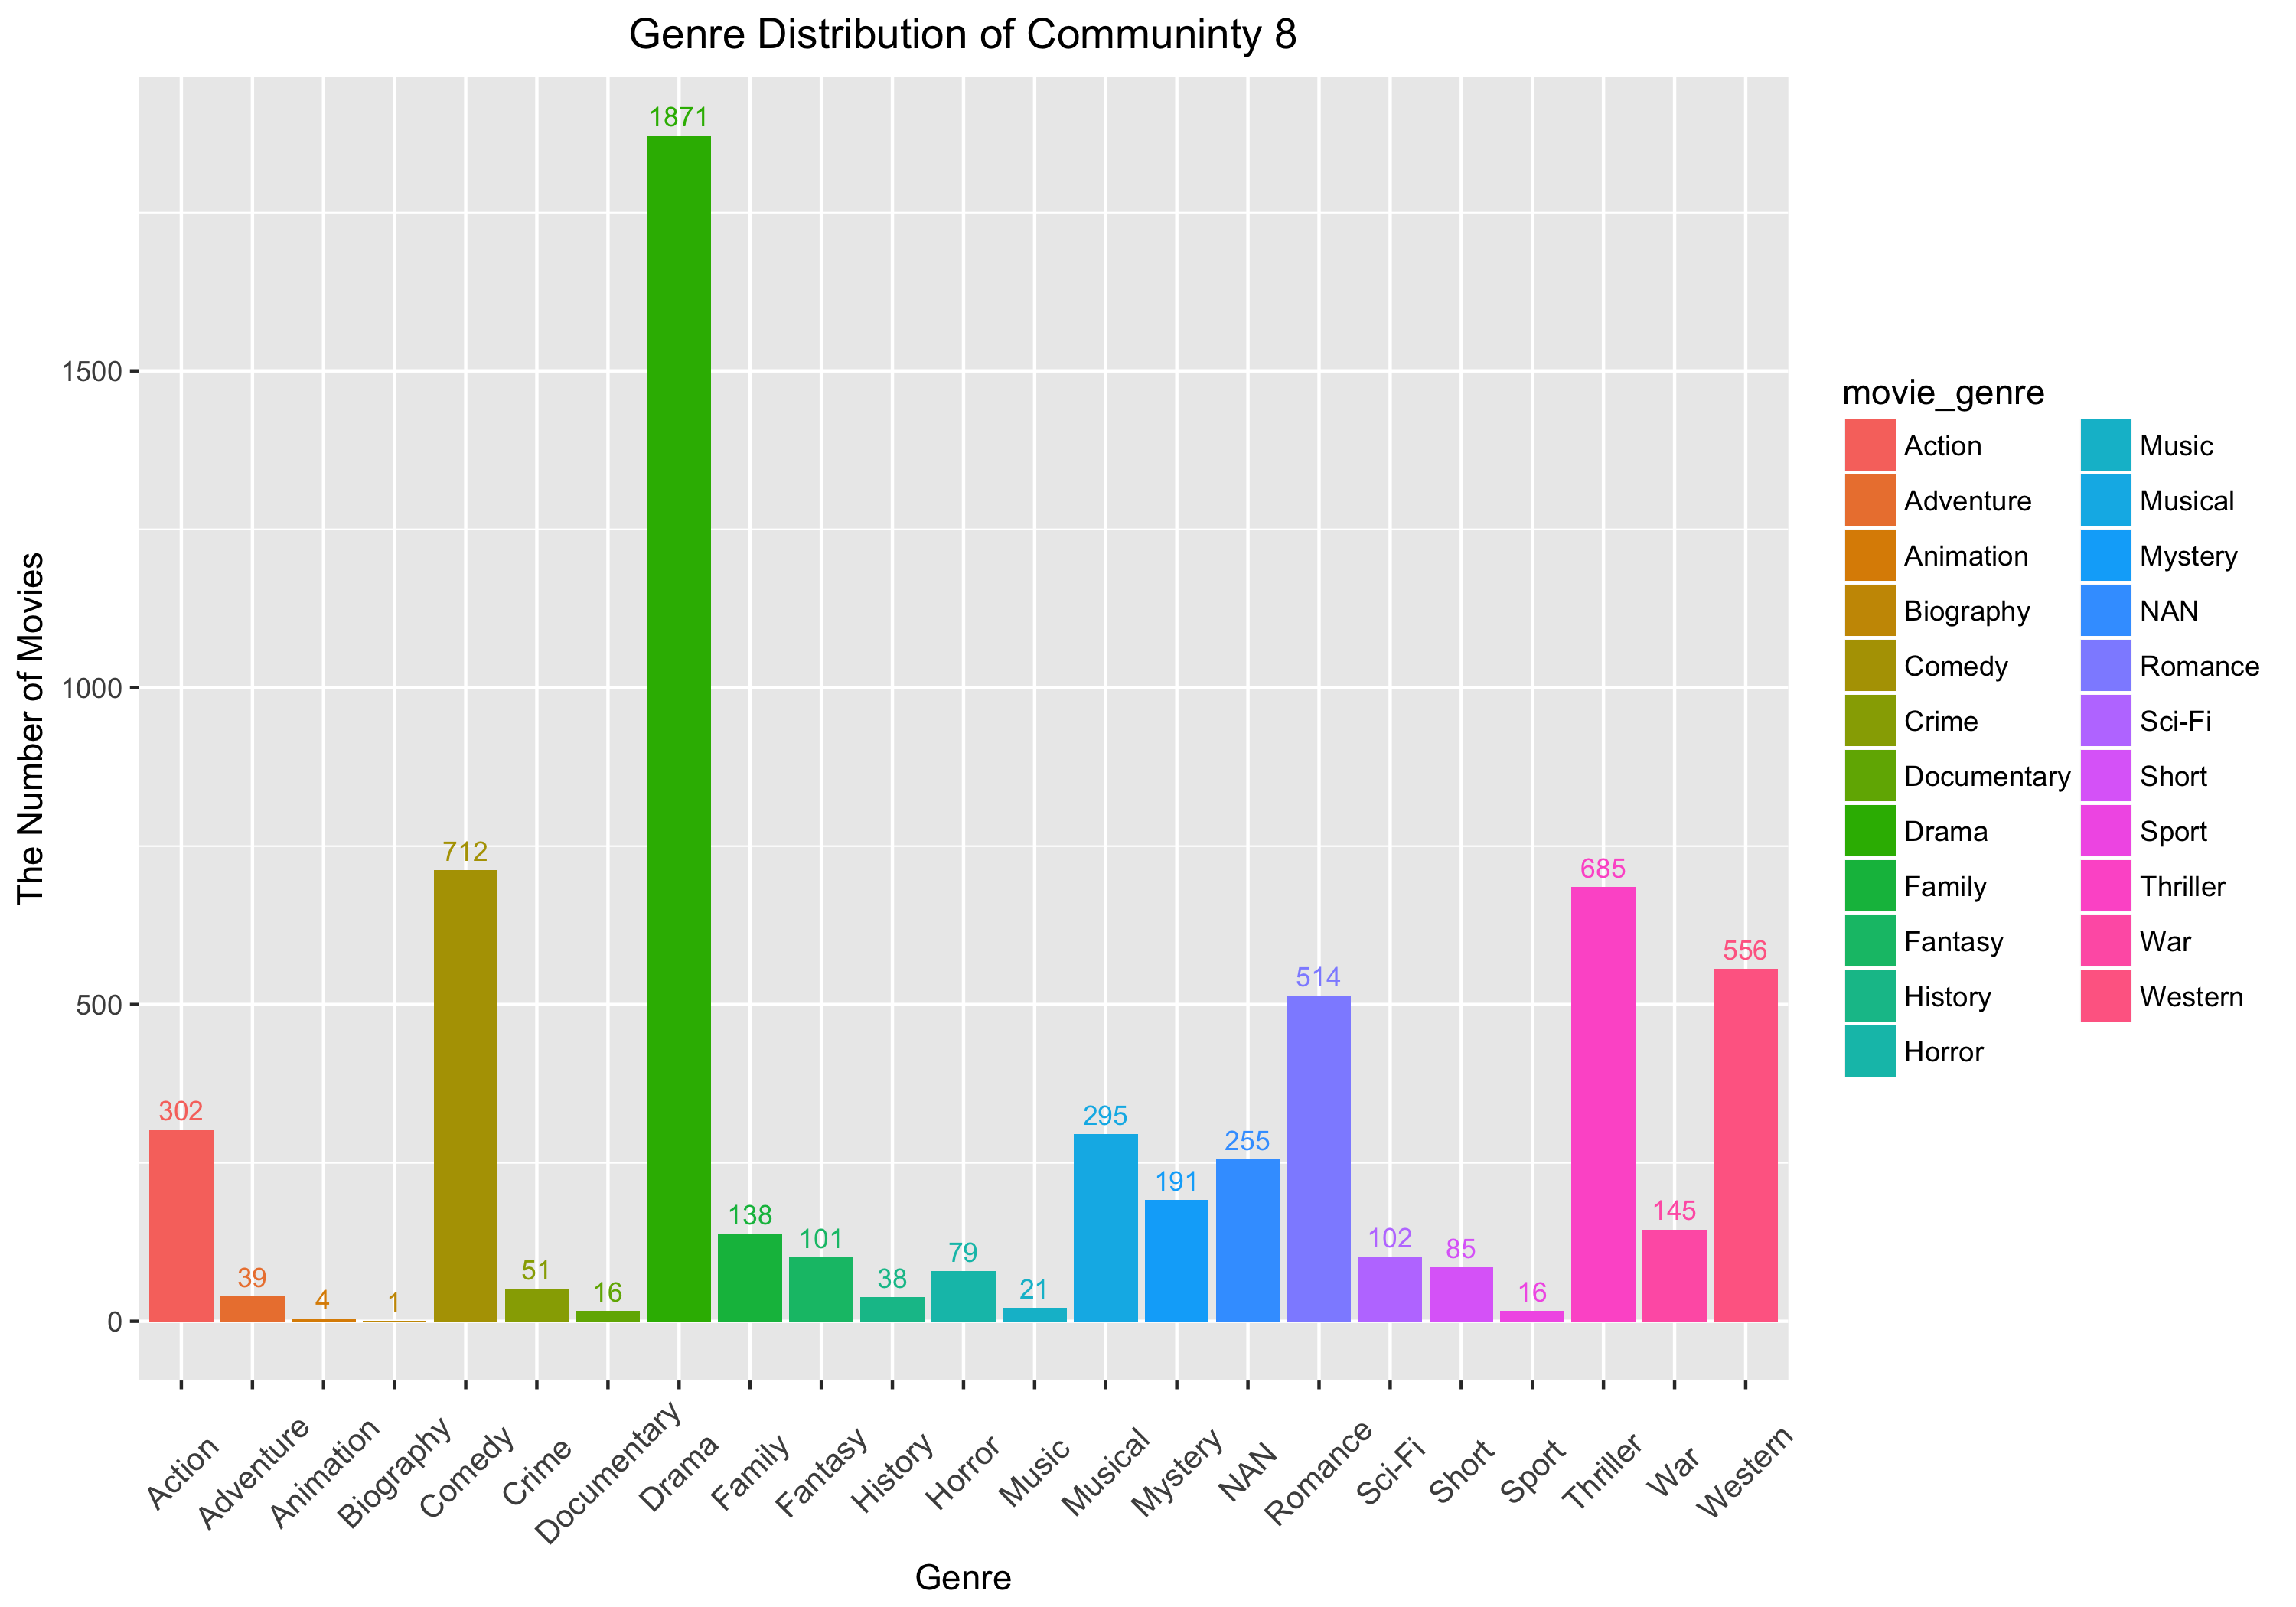
\includegraphics{Figures/community_8.png}}
\caption{Genre Distribution of Community $8$}
\label{fig:Q7_8}
\end{figure}

\begin{figure}[H]
\centering
\scalebox{1}{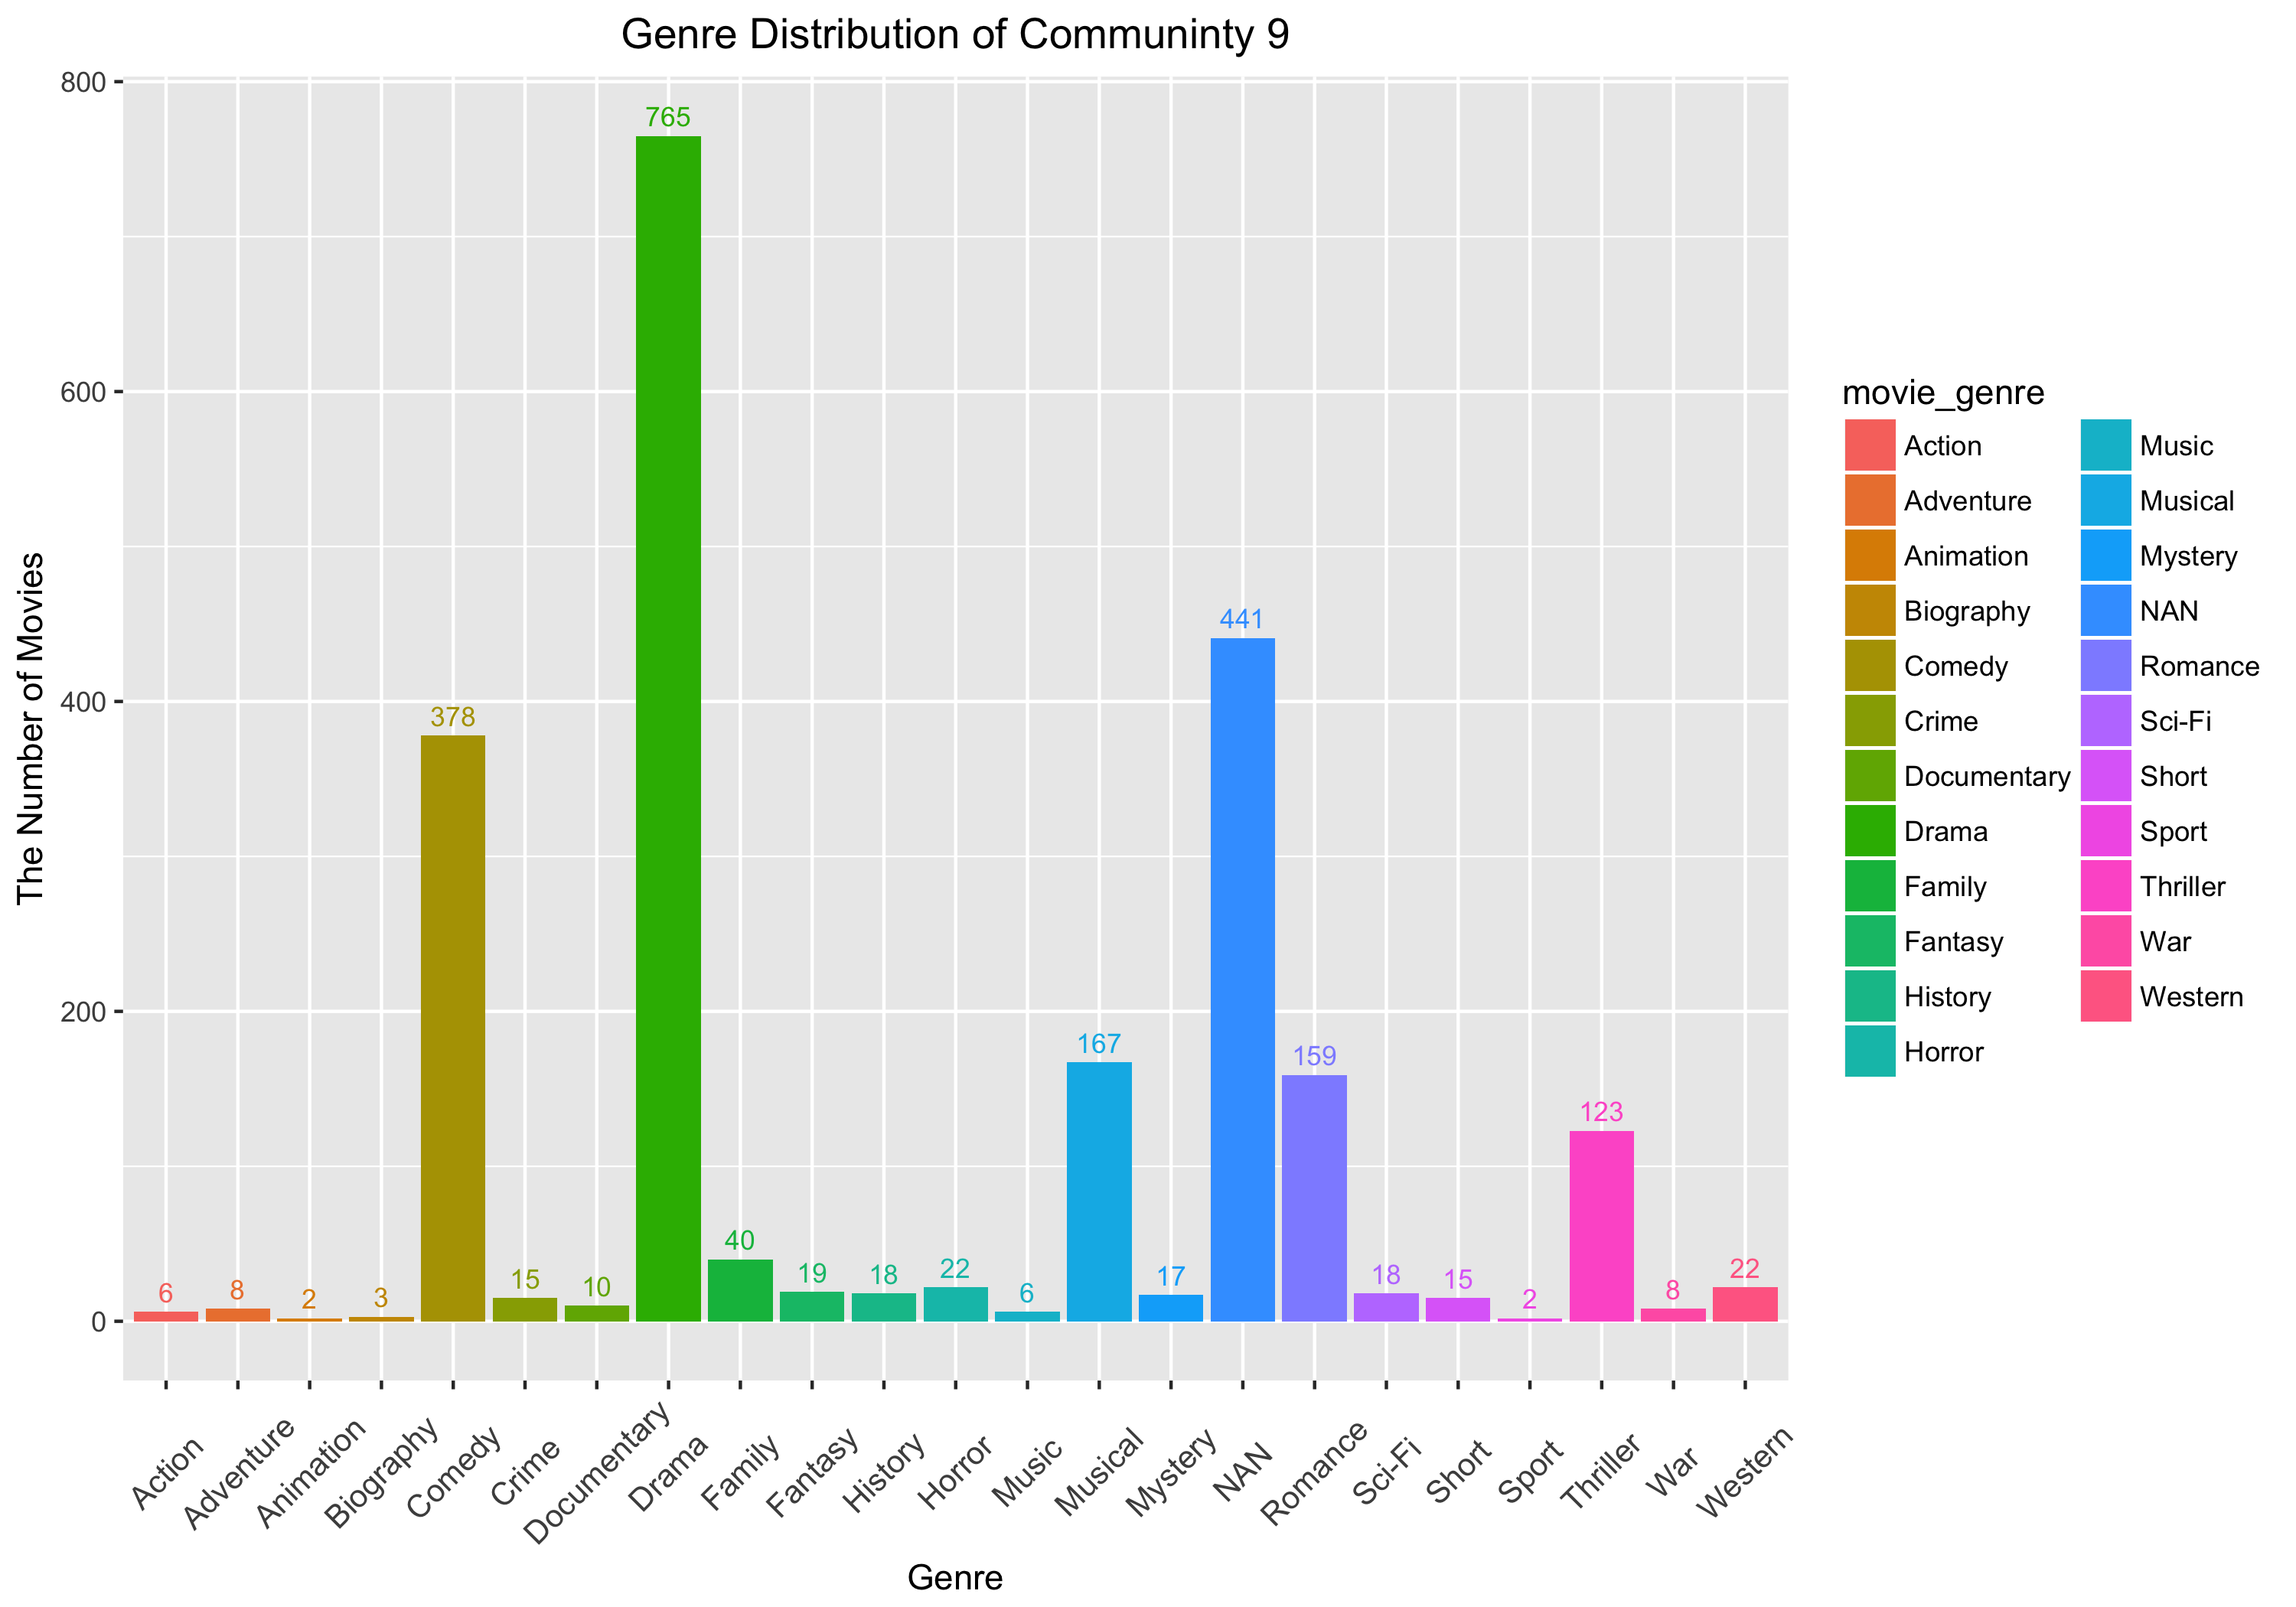
\includegraphics{Figures/community_9.png}}
\caption{Genre Distribution of Community $9$}
\label{fig:Q7_9}
\end{figure}

\begin{figure}[H]
\centering
\scalebox{1}{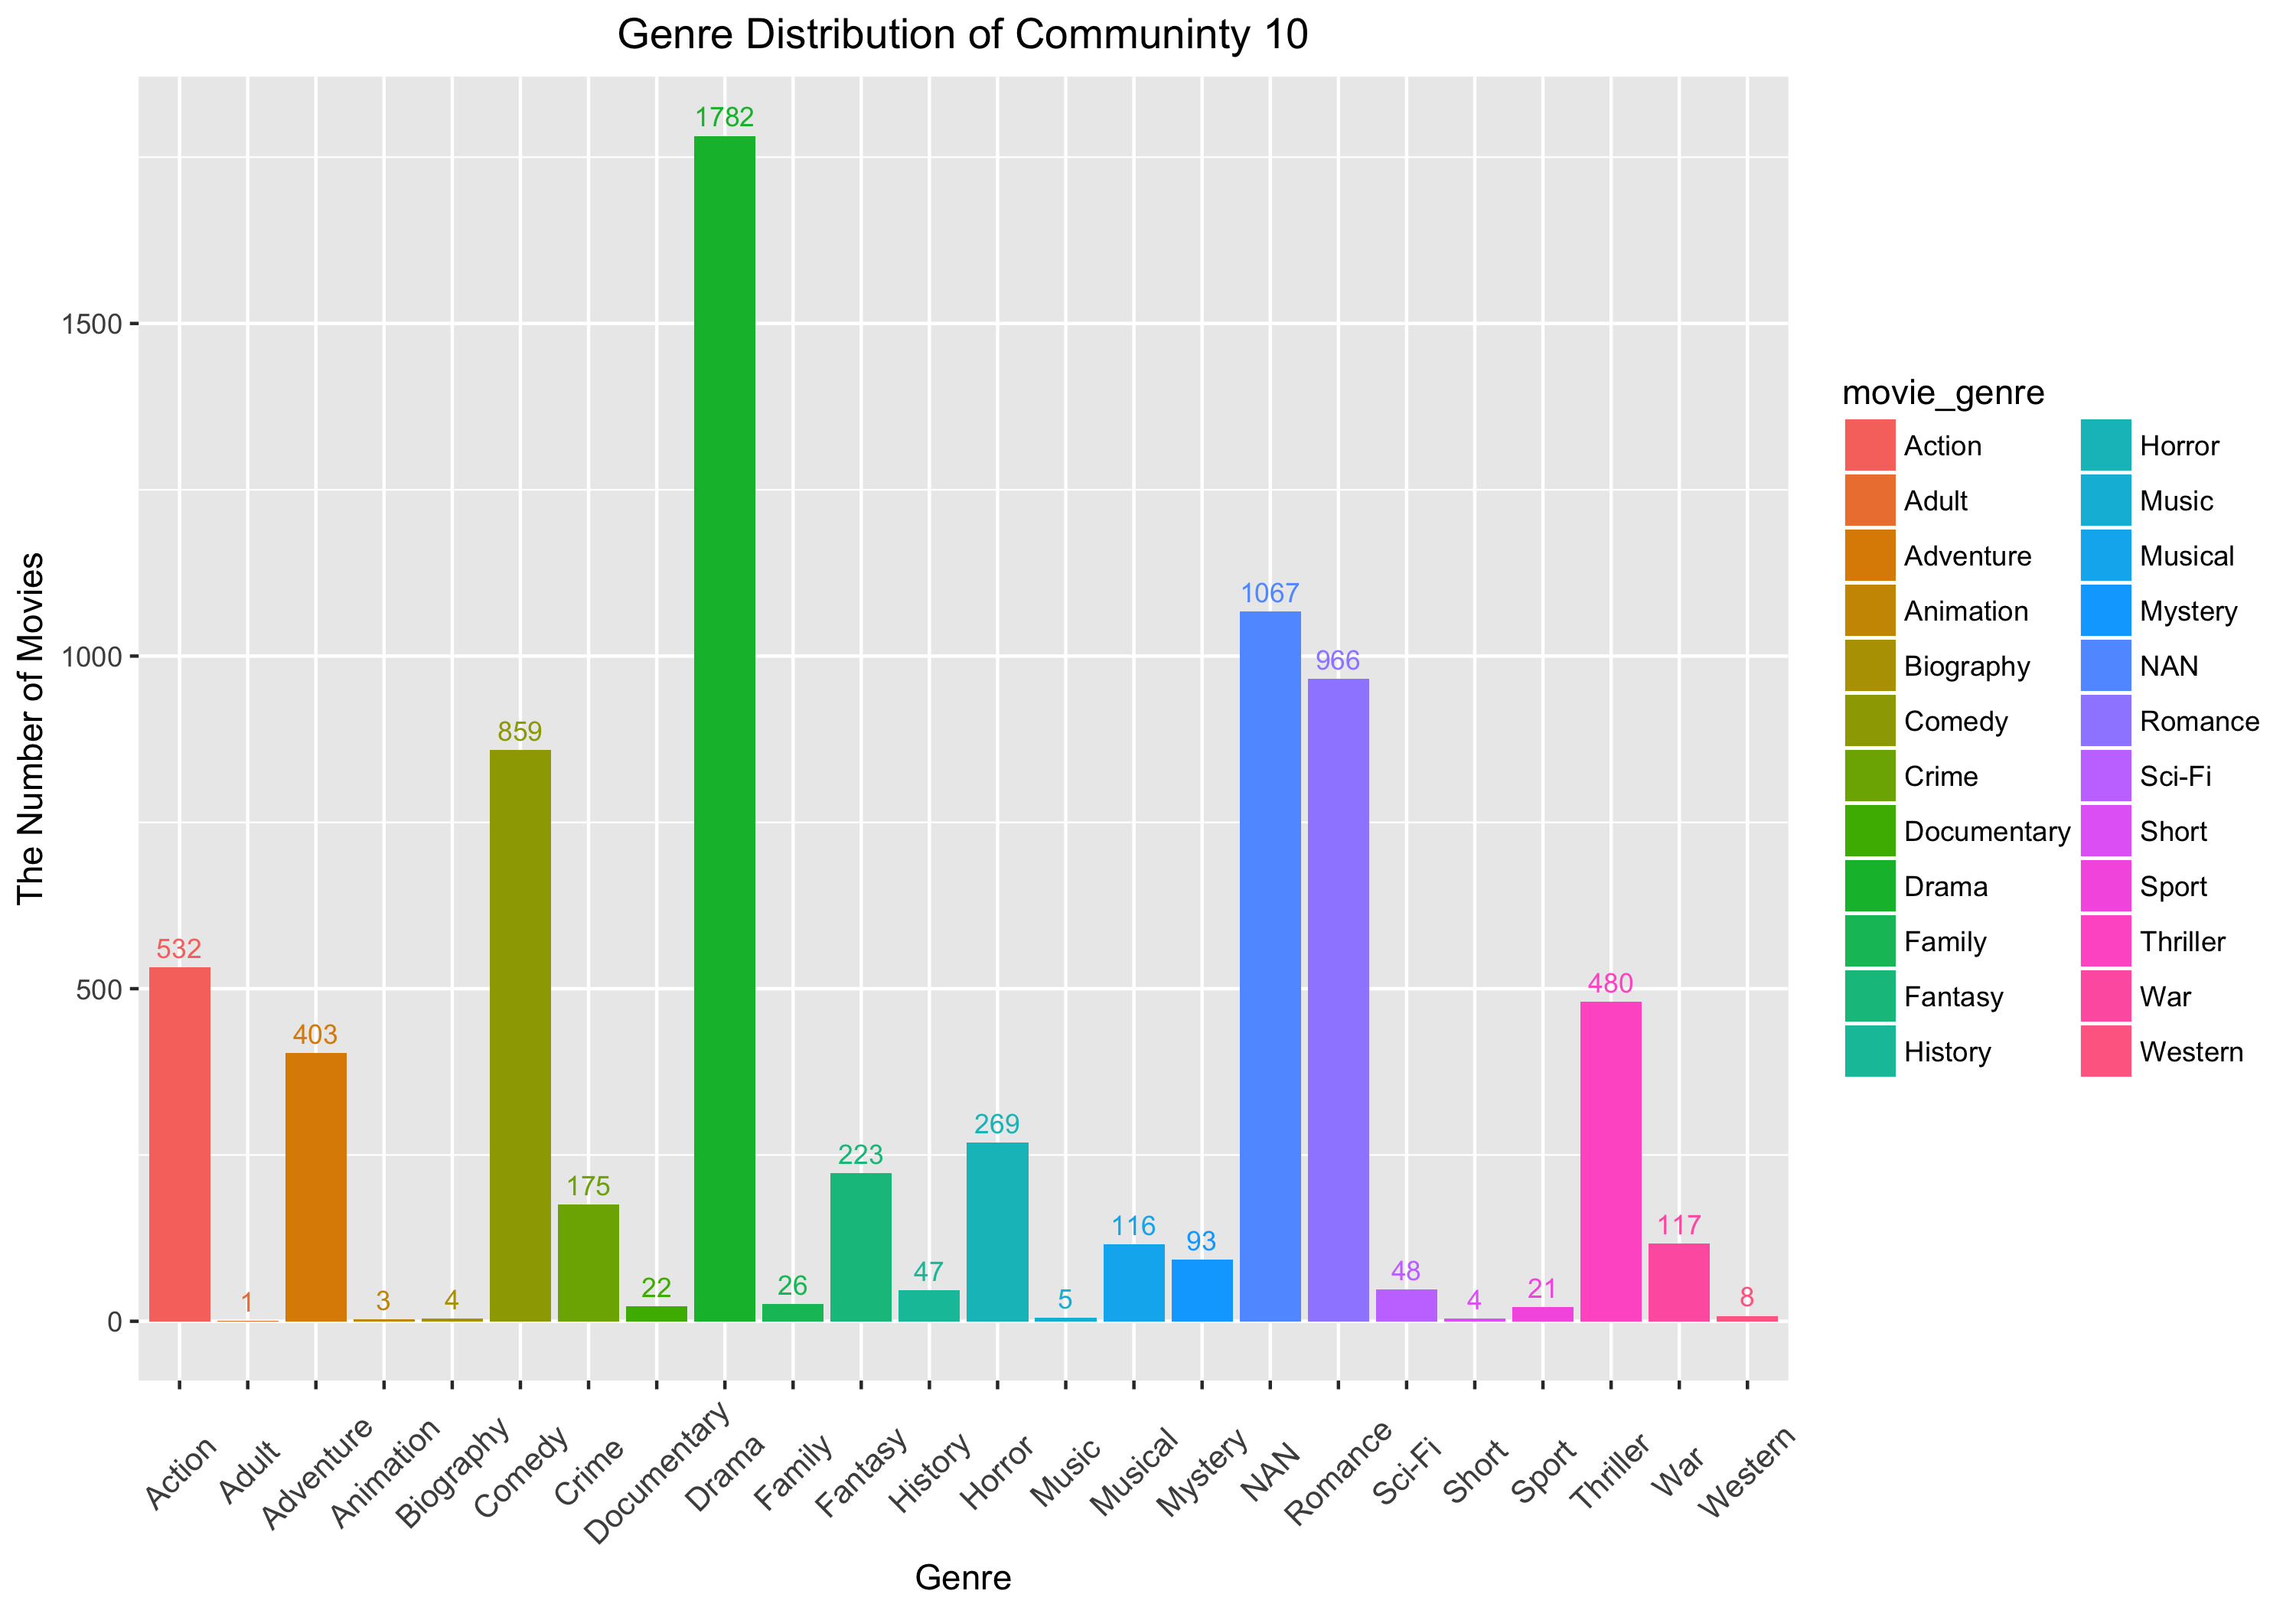
\includegraphics{Figures/community_10.png}}
\caption{Genre Distribution of Community $10$}
\label{fig:Q7_10}
\end{figure}

Based on simple frequency counts, the most dominant genre of each community we got is shown in Table \ref{table_2_1}. As we can see, the genre "Drama" is the dominant genre of 11 communities among 28 communities. This in fact can be easily speculated, because in the movie network, the number of moives marked "Drama" take a high propotion among all the movies. What is worth to notie is that there are some movies without genre mark, which in my charts marked "NAN", and this kind of movie in few communities actually become the category with most number of movies, such as community 28 (the distribution shown in Figure \ref {fig:Q7_11}), where only one movie belongs to "Short" and the rest of movies marked "NAN"; however we need to ignore "NAN" movies, so the donimant genre should be "Short" in this community. 

\begin{table}[H]
\center
\caption{The dominant genre of each community(according to frequency count)}
\scalebox{0.9}{
\begin{tabular}{c|c}
\hline
\textbf{Community ID} & \textbf{the dominant genre}\\\hline
1 & Thriller\\\hline
2 & Short\\\hline
3 & Drama \\\hline
4 & Drama \\\hline
5 & Drama \\\hline
6 & Drama \\\hline
7 & Drama \\\hline
8 & Drama \\\hline
9 & Drama \\\hline
10 & Drama \\\hline
11 & Drama \\\hline
12 & Drama \\\hline
13 & Drama \\\hline
14 & Drama \\\hline
15 & Drama \\\hline
16 & Drama \\\hline
17 & Drama \\\hline
18 & Drama \\\hline
19 & Drama \\\hline
20 & Drama \\\hline
21 & Drama \\\hline
22 & Drama \\\hline
23 & Drama \\\hline
24 & Adult\\\hline
25 & Thriller\\\hline
26 & Short\\\hline
27 & Short\\\hline
28 & Short\\\hline
\end{tabular}}
\label{table_2_1}
\end{table}

\begin{figure}[H]
\centering
\scalebox{1}{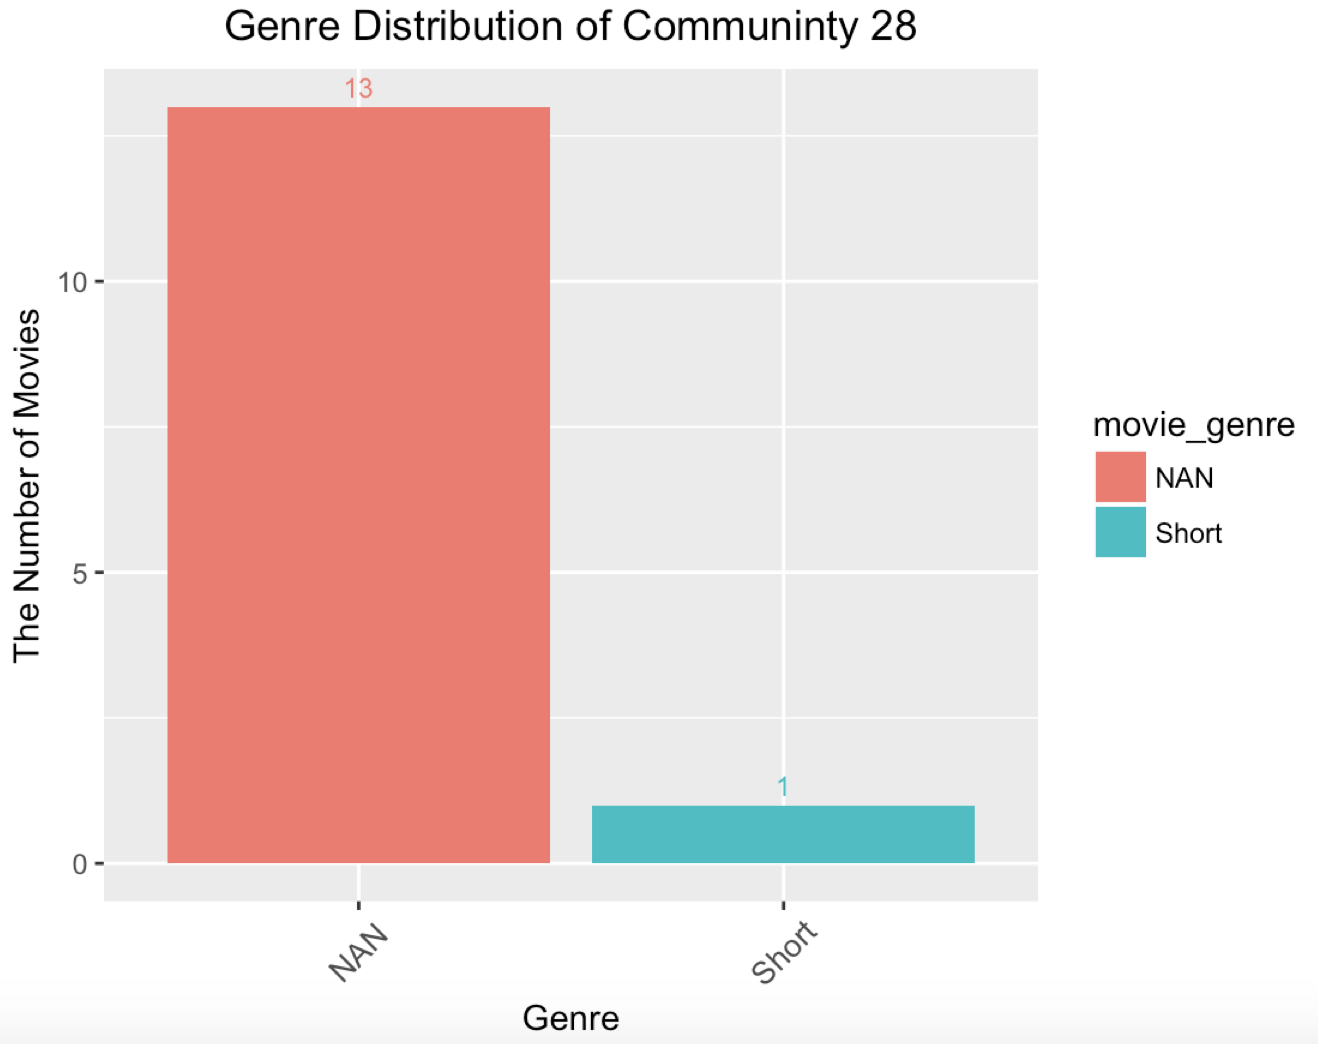
\includegraphics{Figures/community_28.png}}
\caption{Genre Distribution of Community $28$}
\label{fig:Q7_11}
\end{figure}

Based on the measurement of modified score, the dominant genre of each community changes a lot, and the result is shown in Table \ref{table_2_2}. It illustrates that most of the dominant genres we got according to the modified scores are different from the genres we got by simply couting the frequency of genre within the community. Interestingly, there do exist some communities hold the same dominant genre and all of them have comparably fewer movies than other communities. To be sepecific, the number of movies in these communities is in the range of (10,20). In addition, the frequency of the dominant genre in these communities is far more higer than other genres. For instance, we also plotted community with ID=24 and ID=25, shown in Figure \ref{fig:Q8_1} and \ref{fig:Q8_2}. In fact, this is reasonable because in these kinds of communities, $p(i)$ of the dominant genre(the genre has the highest frequency) is much bigger than other genres within the community, which can play a dominant role of the score function. Moreover, some of the genres in these kinds of communities have only one occurency, which makes $c(i)$ equals to 1 and then $ln(c(i))$ equals to 0, so that the score will be 0. On the contrary, for those communities whose dominant genre differ from different measurement, they generally include large number of movies, and may have genres holding the similar frequency wihthin the communiy. For instance, we could observe the genre distribution of community with ID=6 (Figure \ref{fig:Q7_6}), the dominant genre changes from "Drama"(the most frequent genre) to "Comedy"(the third frequent genre). This is easy to understand since the score function consider the fraction of genre within community and also in whole dataset, which is equvalent to multiply some coefficients to the exact frequency of the genre, this somehow makes the score bigger or smaller comparing to the exact frequency. Therefore, the dominant genre of these kinds of community changes. 

\begin{table}[H]
\center
\caption{The dominant genre of each community(according to modified score)}
\scalebox{0.9}{
\begin{tabular}{c|c}
\hline
\textbf{Community ID} & \textbf{the dominant genre}\\\hline
1 & Adult \\\hline
2 & Film-Noir \\\hline
3 & War \\\hline
4 & Crime \\\hline
5 & Family \\\hline
6 & Comedy \\\hline
7 & Family \\\hline
8 & Musical \\\hline
9 & Musical \\\hline
10 & Adventure \\\hline
11 & Family \\\hline
12 & Romance \\\hline
13 & War \\\hline
14 & Adventure \\\hline
15 & Comedy \\\hline
16 & Musical \\\hline
17 & Action \\\hline
18 & Drama \\\hline
19 & Fantasy \\\hline
20 & Comedy \\\hline
21 & Action \\\hline
22 & Romance \\\hline
23 & Short \\\hline
24 & Adult \\\hline
25 & Thriller \\\hline
26 & Short \\\hline
27 & Short \\\hline
28 & Short \\\hline
\end{tabular}}
\label{table_2_2}
\end{table}


\begin{figure}
\centering
\begin{minipage}[h]{0.48\textwidth}
\centering
\scalebox{1}{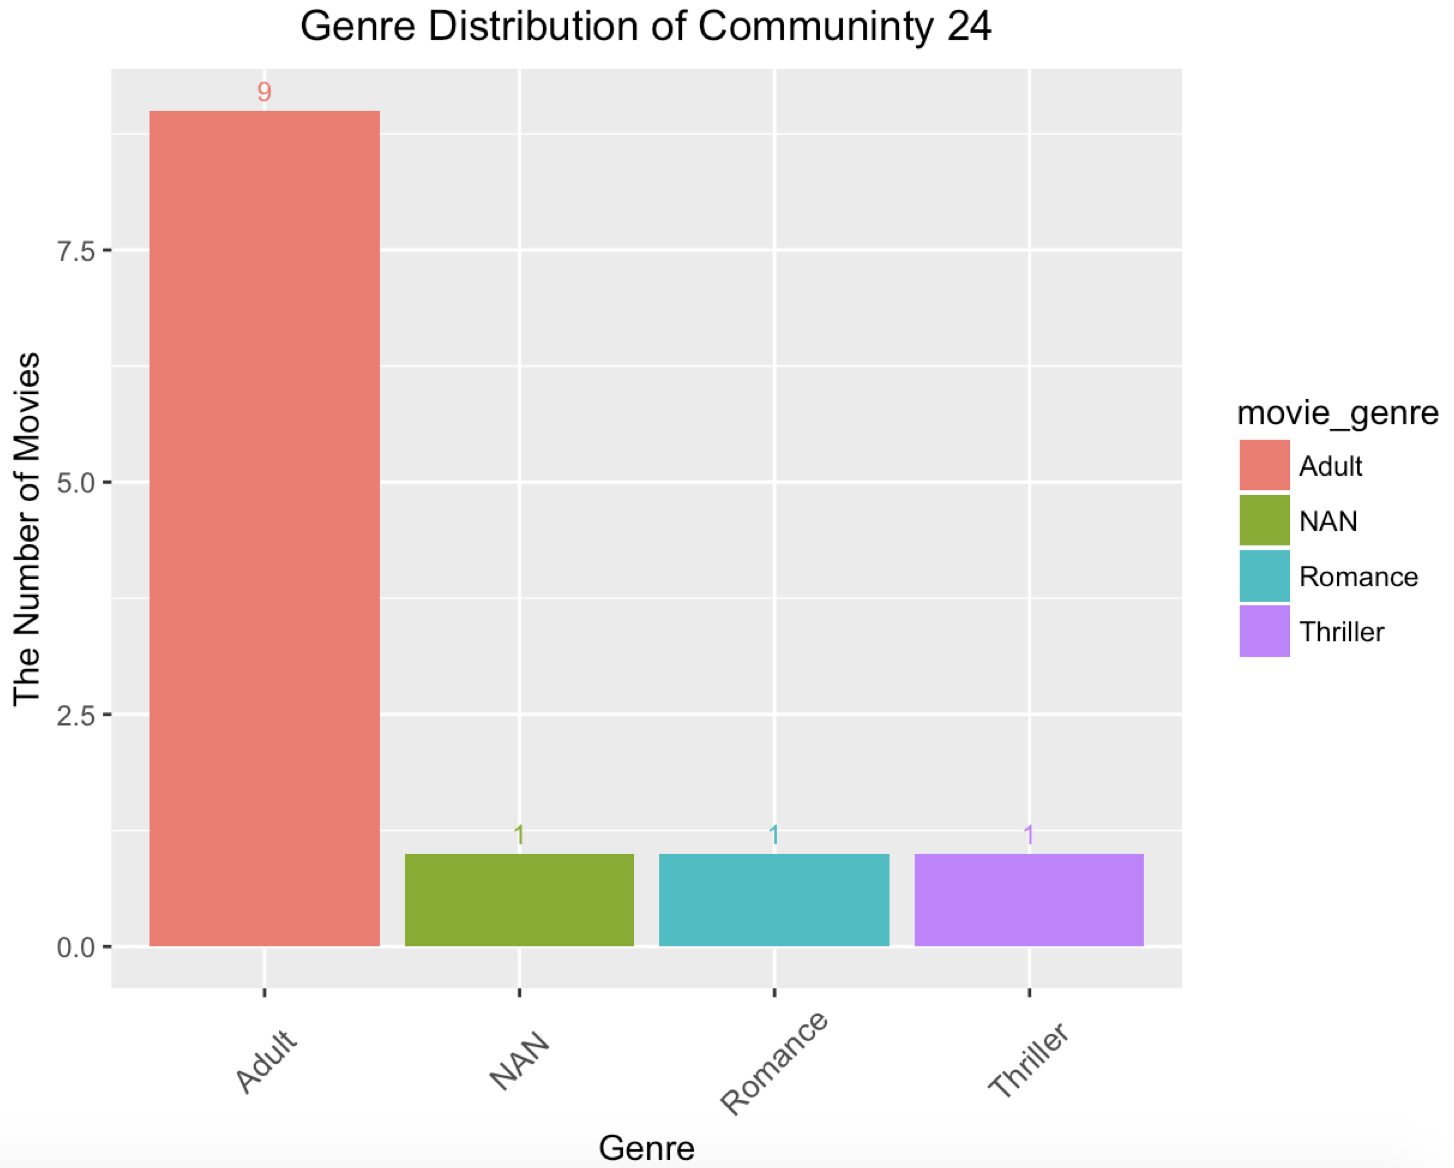
\includegraphics{Figures/community_24.png}}
\caption{Genre Distribution of Community $24$}
\label{fig:Q8_1}
\end{minipage}
\begin{minipage}[h]{0.48\textwidth}
\centering
\scalebox{1}{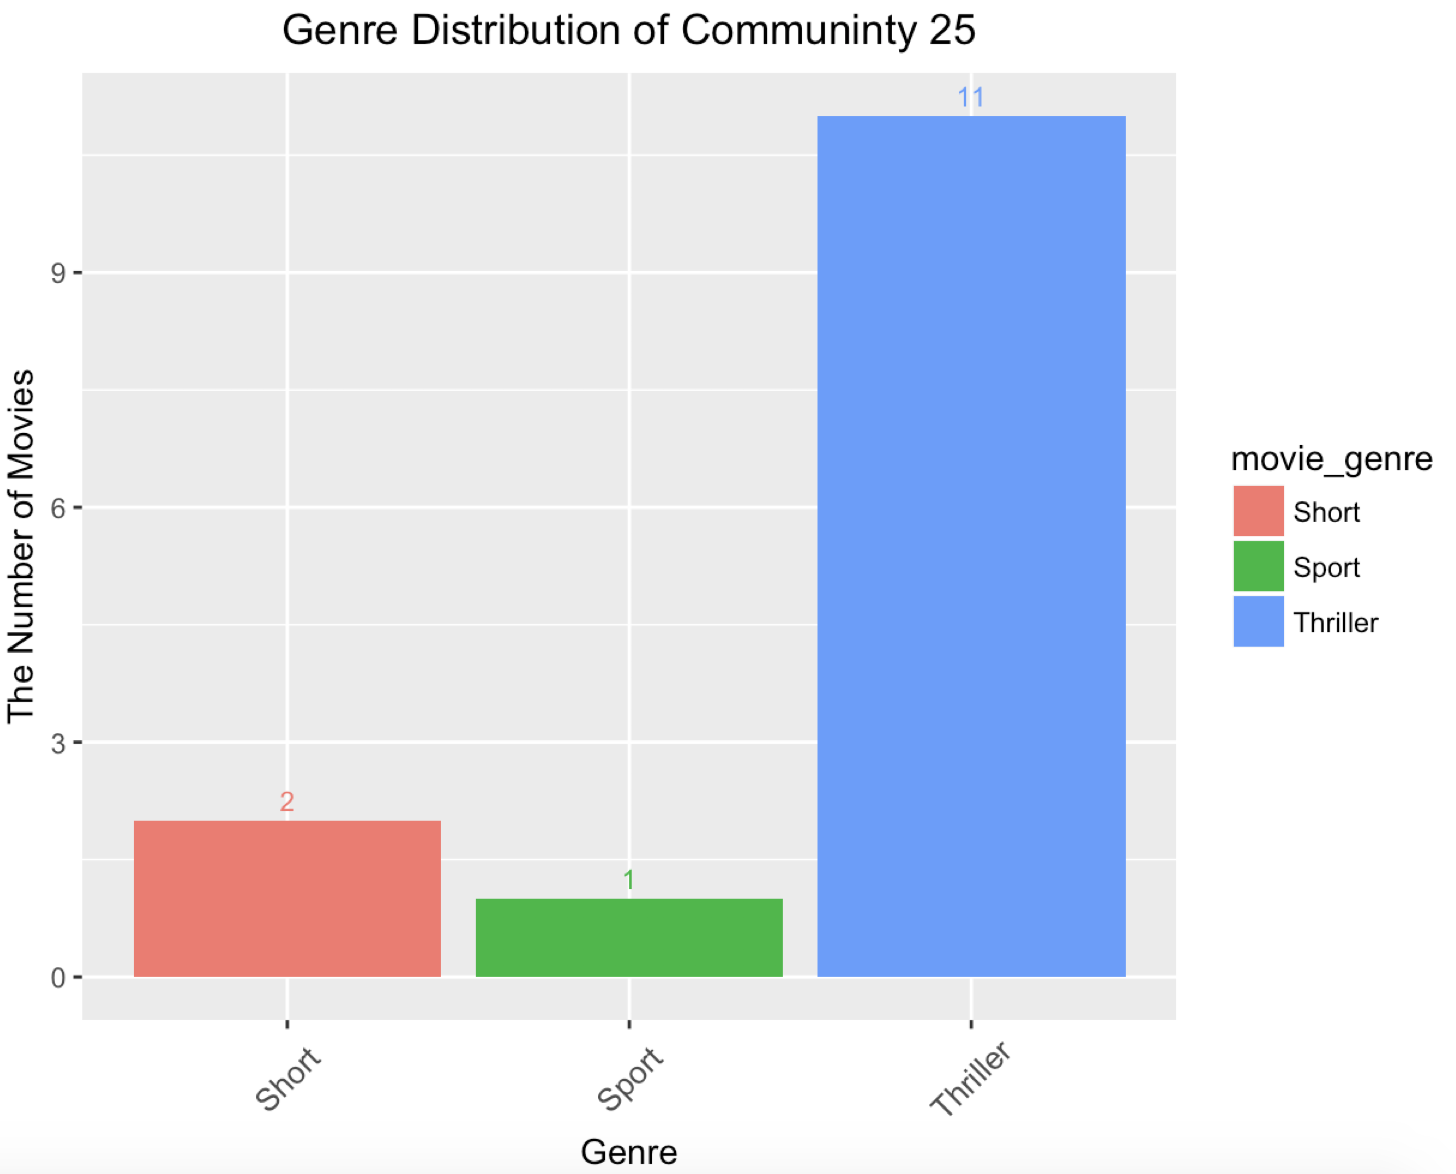
\includegraphics{Figures/community_25.png}}
\caption{Genre Distribution of Community $25$}
\label{fig:Q8_2}
\end{minipage}
\end{figure}


We chose community(ID=24) who includes 12 movies to further study the correlation among actors, movies and genres. Table \ref{table_2_3} shows the basic informaiton of this community, while Table \ref{table_2_4} and Table \ref{table_2_5} list the ID and Name mapping correlation in movies and actors respectively.

\begin{table}[H]
\center
\caption{Basic Information of Community 24}
\scalebox{0.9}{
\begin{tabular}{r|c|c}
\hline
\textbf{Movie ID} & \textbf{Genre} & \textbf{Actor ID}\\\hline
93381 & Thriller & 4196,19653,26390,35604,45645,56587,60399,66920\\\hline
151826 & Adult & 8242,20204,21948,60399,89726\\\hline
151830 & Adult & 8242,21948,60399,93363,111639\\\hline
151831 & Adult & 8242,21948,32885,60399,68271,83742\\\hline
151832 & Adult & 8242,21948,32885,60399,83742\\\hline
151838 & Adult & 8242,24483,65193,68271,102098\\\hline
151840 & Adult & 8242,20204,21948,60399,89726,11639\\\hline
151841 & Romance & 8242,21948,32885,68271,83742\\\hline
151842 & Adult & 8242,20204,21948,60399,83742,111639\\\hline
151845 & NAN & 8242,21948,32885,60399,69507\\\hline
251442 & Adult & 20204,32885,60399,68271,93363\\\hline
251446 & Adult & 20204,21948,32885,89726,102098\\\hline

\end{tabular}}
\label{table_2_3}
\end{table}


\begin{table}[H]
\center
\caption{Movie ID mapping to Movie Name (for community 24)}
\scalebox{0.9}{
\begin{tabular}{c|c}
\hline
\textbf{Movie ID} & \textbf{Movie Name}\\\hline
93381 & Baise-moi (2000)\\\hline
151826 & Aleska \& Angelika: Pornochic 21 (2011)\\\hline
151830 & Dorcel Airlines: Paris/New York (2010)\\\hline
151831 & Initiation of Lou Charmelle (2010)\\\hline
151832 & Jade, Secretaire de Luxe (2011)\\\hline
151838 & Maximum Orgy, spÈcial pin-up (2012)\\\hline
151840 & Russian Institute: Anal Lesson (2010)\\\hline
151841 & Soubrettes Services (2010)\\\hline
151842 & Soubrettes Services: Special Stars (2010)\\\hline
151845 & Story of MÈgane (2008)\\\hline
251442 & Hard Intrusion (2007)\\\hline
251446 & Russian Institute Lesson 16: Lolitas (2011)\\\hline
\end{tabular}}
\label{table_2_4}
\end{table}



\begin{table}[H]
\center
\caption{Actor ID mapping to Actor Name (for community 24)}
\scalebox{0.9}{
\begin{tabular}{c|c}
\hline
\textbf{Actor ID} & \textbf{Actor Name}\\\hline
4196 & Barrio, Sebastian (I)\\\hline
8242 & Brossman, James\\\hline
19653 & Embarek, Ouassini\\\hline
20204 & Evil, Leny\\\hline
21948 & Forte, Alex\\\hline
24483 & Giotto, Lauro\\\hline
26390 & Gustave, HervÈ P.\\\hline
32885 & JPX\\\hline
35604 & Kodjo Topou, Patrick\\\hline
45645 & MinÈo, Jean-Marc\\\hline
56587 & Rioufol, Marc\\\hline
60399 & Scott, Ian (III)\\\hline
65193 & SX, Bruno\\\hline
66920 & Titof\\\hline
68271 & Uhl, George\\\hline
69507 & Vidal, Nacho (I)\\\hline
83742 & Dollar, Cindy\\\hline
89726 & Hope, Cindy\\\hline
93363 & Lafitte, Yasmine\\\hline
102098 & Polina, Anna\\\hline
111639 & White, Tarra\\\hline
\end{tabular}}
\label{table_2_5}
\end{table}


The bipartite graph we got is shown in Figure \ref{fig:Q8_3}, where red vertices represen the actors and blue vertices represent the movies.

\begin{figure}[H]
\centering
\scalebox{1}{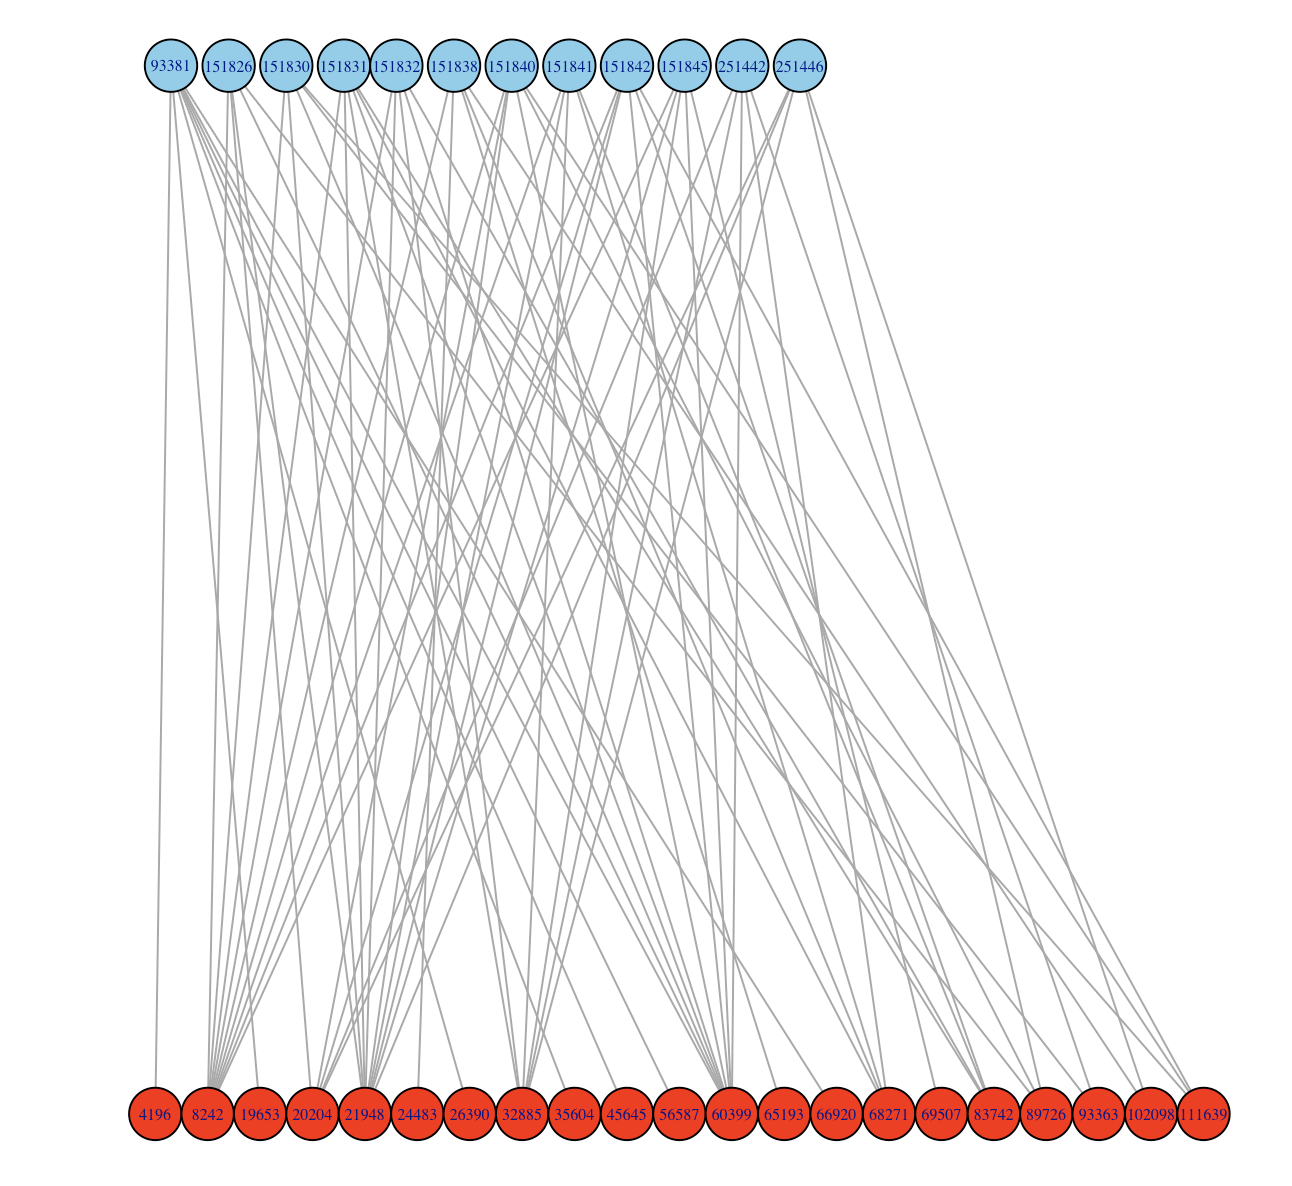
\includegraphics{Figures/comm24_bipartite_grpah.png}}
\caption{Bipartite Graph of Movies and Actors in Community 24}
\label{fig:Q8_3}
\end{figure}

After statistical analysis, we found that the three most important actors‘ID are 8242 21948 60399. Then, we searched all the movies these three actors have ever acted. Not surprisingly, the dominant genre of these movies is also "Adult", the same as the dominant genre of the community 24 that we got in we got in 8(a) and 8(b). That is to say, these three most important actors involved in the same kind of movies, which determines the community and the dominant genre of the community. In other words, the community we got by the Fast Greedy algorithm helps us find movies in same(or similar) genre. 





\subsection{Neighborhood analysis of movies}
In this section, we analyzed the relationship between the rating of a movie and its neighbors. Specifically, we mainly investigated the following three movies.
\begin{itemize}
\item Batman v Spiderman: Dawn of Justice (2016); Rating $6.6$;
\item Mission: Impossible - Rogue Nation (2015); Rating $7.4$;
\item Minions (2015); Rating $6.4$.
\end{itemize}

\textcolor{red}{\textbf{Question 9:} For each of the movie listed above, extract it's neighbors and plot the distribution of the available ratings of the movies in the neighborhood. Is the average rating of the movies in the neighborhood similar to the rating of the movie whose neighbors have been extracted? In this question, you should have $3$ plots.}

After extracting the neighbors of the above three movies and computing the mean of the available ratings in the neighbor vertices, we obtained the Fig. \ref{fig:distribution_1}, \ref{fig:distribution_2}, and \ref{fig:distribution_3}. The average ratings of the neighbor network of the above three movies are shown in Table. \ref{table:no_comm}. It can be seen that, with this scheme, the average rating in the neighbor network is not very similar to the actual rating of the movie.

\begin{table}[H]
\center
\caption{Average rating vs. actual rating of the three movies}
\scalebox{0.9}{
\begin{tabular}{c|c|c}
\hline
\textbf{Movie Name} & \textbf{Actual Rating} & \textbf{Average Rating}\\\hline
Batman v Spiderman: Dawn of Justice (2016) & $6.6$ & $6.4$\\
Mission: Impossible - Rogue Nation (2015) & $7.4$ & $6.3$\\
Minions (2015) & $6.4$ & $6.9$\\\hline

\end{tabular}}
\label{table:no_comm}
\end{table}

\begin{figure}
\centering
\begin{minipage}[H]{0.48\textwidth}
\centering
\scalebox{1}{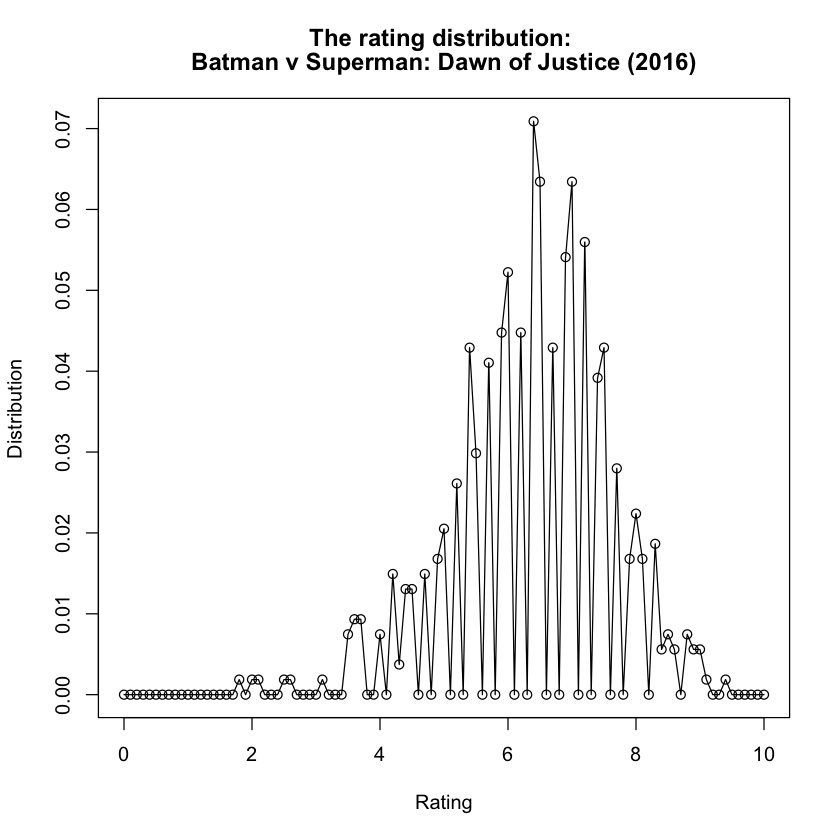
\includegraphics{Figures/hj_01.png}}
\caption{The rating distribution of the neighbor network\\Batman v Spiderman: Dawn of Justice (2016)}
\label{fig:distribution_1}
\end{minipage}
\begin{minipage}[H]{0.48\textwidth}
\centering
\scalebox{1}{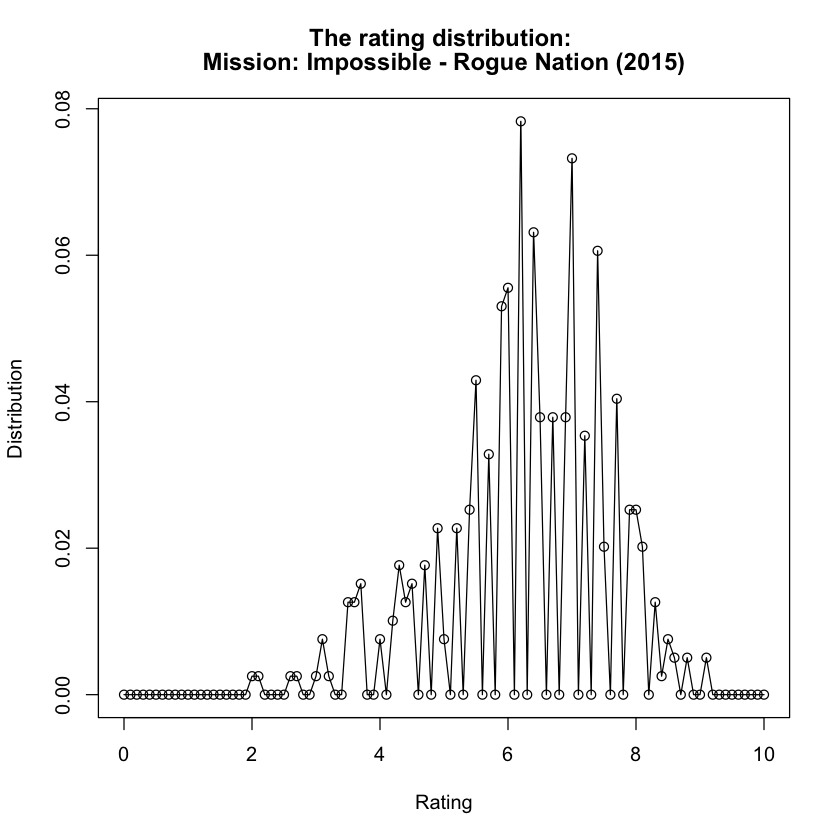
\includegraphics{Figures/hj_02.png}}
\caption{The rating distribution of the neighbor network\\Mission: Impossible - Rogue Nation (2015)}
\label{fig:distribution_2}
\end{minipage}
\end{figure}


\begin{figure}
\centering
\begin{minipage}[H]{0.48\textwidth}
\centering
\scalebox{1}{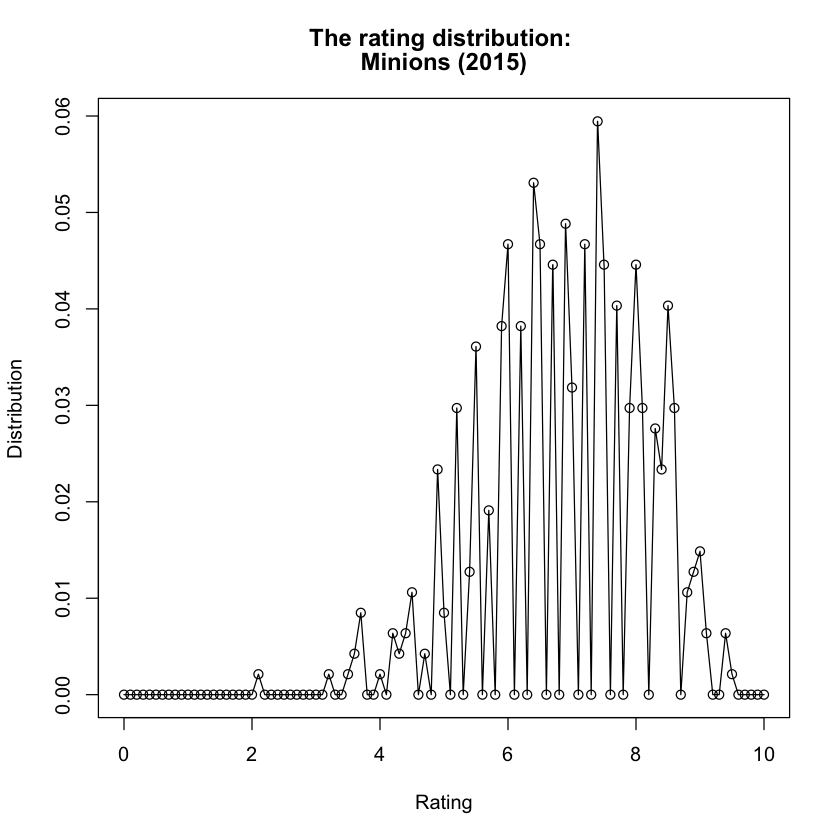
\includegraphics{Figures/hj_03.png}}
\caption{The rating distribution of the neighbor network\\Minions (2015)}
\label{fig:distribution_3}
\end{minipage}
\begin{minipage}[H]{0.48\textwidth}
\centering
\scalebox{1}{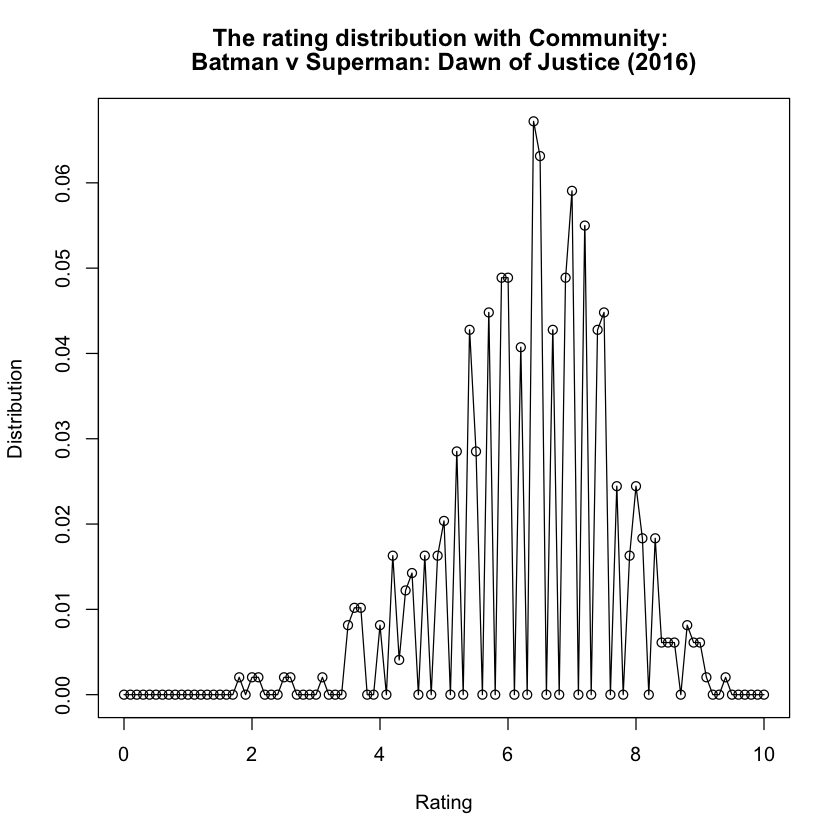
\includegraphics{Figures/hj_04.png}}
\caption{The rating distribution of the neighbor network with the same community\\Batman v Spiderman: Dawn of Justice (2016)}
\label{fig:distribution_4}
\end{minipage}
\end{figure}

\begin{figure}
\centering
\begin{minipage}[H]{0.48\textwidth}
\centering
\scalebox{1}{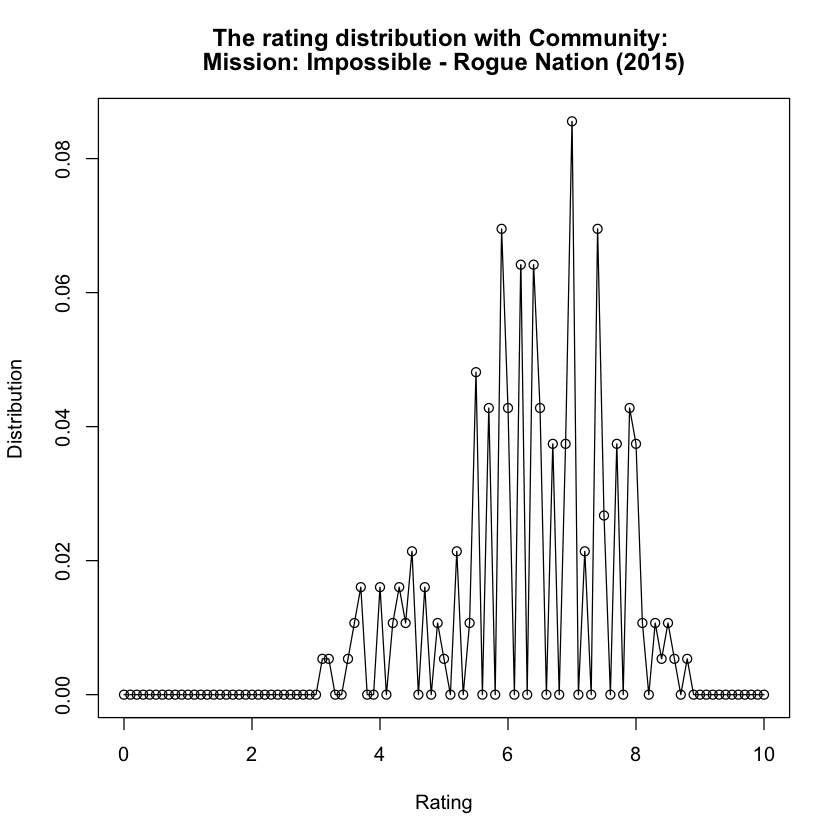
\includegraphics{Figures/hj_05.png}}
\caption{The rating distribution of the neighbor network with the same community\\Mission: Impossible - Rogue Nation (2015)}
\label{fig:distribution_5}
\end{minipage}
\begin{minipage}[H]{0.48\textwidth}
\centering
\scalebox{1}{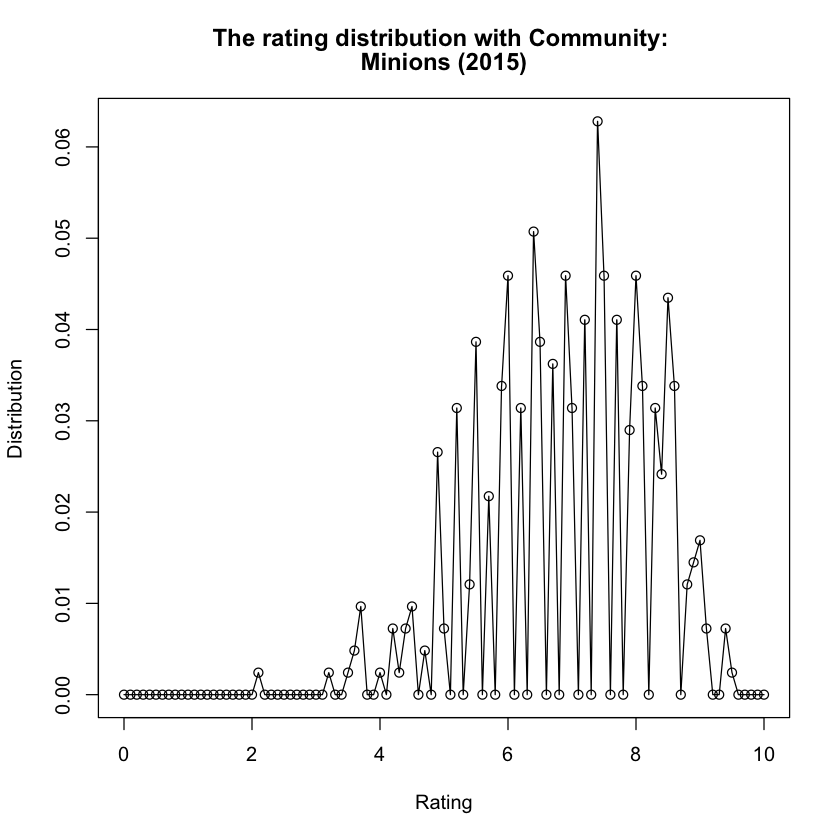
\includegraphics{Figures/hj_06.png}}
\caption{The rating distribution of the neighbor network with the same community\\Minions (2015)}
\label{fig:distribution_6}
\end{minipage}
\end{figure}


\textcolor{red}{\textbf{Question 10:} Repeat question $9$, but now restrict the neighborhood to consist of movies from the same community. Is there a better match between the average rating of the movies in the restricted neighborhood and the rating of the movie whose neighbors have been extracted. In this question, you should have $3$ plots.}

After constraining the community, the rating distributions we obrtained are shown in Fig. \ref{fig:distribution_4}, \ref{fig:distribution_5}, and \ref{fig:distribution_6}. The average ratings of the neighbor network of the above three movies are shown in Table. \ref{table:with_comm}. It can be seen that, after contraining the neighbor vertices are in the same community, the average rating in the neighbor network is still not very similar to the actual rating of the movie.

\begin{table}[H]
\center
\caption{Average rating vs. actual rating of the three movies, with community considered}
\scalebox{0.9}{
\begin{tabular}{c|c|c}
\hline
\textbf{Movie Name} & \textbf{Actual Rating} & \textbf{Average Rating}\\\hline
Batman v Spiderman: Dawn of Justice (2016) & $6.6$ & $6.4$\\
Mission: Impossible - Rogue Nation (2015) & $7.4$ & $6.4$\\
Minions (2015) & $6.4$ & $6.9$\\\hline
\end{tabular}}
\label{table:with_comm}
\end{table}

\textcolor{red}{\textbf{Question 11:} For each of the movies listed above, extract it's top $5$ neighbors and also report the community membership of the top $5$ neighbors. In this question, the sorting is done based on the edge weights.}

After sorting the edge values in decreasing order in the neighbor network, the result is shown in Table. \ref{table:top_movies}.

\begin{table}[H]
\center
\caption{Top $5$ neighbors of the three movies}
\scalebox{0.9}{
\begin{tabular}{c|c|c}
\hline
\textbf{Movie Name} & \textbf{Top $5$ Neighbors} & \textbf{Community ID}\\\hline
\multirow{5}{*}{\makecell{Batman v Spiderman: \\Dawn of Justice (2016)}} & Eloise (2015) & $1$\\
 & The Justice League Part One (2017) & $1$\\
 & Into the Storm (2014) & $1$\\
 & Love and Honor (2013) & $1$\\
 & Man of Steel (2013) & $1$\\\hline
\multirow{5}{*}{\makecell{Mission: Impossible -\\ Rogue Nation (2015)}} & Fan (2015) & $5$\\
 & Phantom (2015) & $5$\\
 & Breaking the Bank (2014) & $4$\\
 & Suffragette (2015) & $4$\\
 & Now You See Me: The Second Act (2016) & $1$\\\hline
\multirow{5}{*}{Minions (2015)} & The Lorax (2012) & $1$\\
 & Inside Out (2015) & $1$\\
 & Up (2009) & $1$\\
 & Despicable Me 2 (2013) & $1$\\
 & Surf's Up (2007) & $1$\\\hline
\end{tabular}}
\label{table:top_movies}
\end{table}


\subsection{Predicting ratings of movies}
In this section, we explore how to use different models to predict the rating of a movie. Still, we try to predict the ratings of the following three movies.

\begin{itemize}
\item Batman v Spiderman: Dawn of Justice (2016); 
\item Mission: Impossible - Rogue Nation (2015);
\item Minions (2015).
\end{itemize}

\textcolor{red}{
    \textbf{Question 12:} Train a regression model to predict the ratings of movies: for the training set you can pick any subset of movies with available ratings as the target variables; you have to specify the exact feature set that you use to train the regression model and report the root mean squared error (RMSE). Now use this trained model to predict the ratings of the $3$ movies listed above (which obviously should not be included in your training data).
}



\textcolor{red}{
    \textbf{Question 13:} Create a bipartite graph following the procedure described above. Determine and justify a metric for assigning a weight to each actor. Then, predict the ratings of the $3$ movies using the weights of the actors in the bipartite graph. Report the RMSE. Is this rating mechanism better than the one in question $12$? Justify your answer.
}

\end{document}







